% !TEX enableShellEscape = yes
% (The above line makes atom-latex compile with -shell-escape for
% minted, and is just ignored by other systems.)


%====================================================
% Please read the README.txt file first.
%====================================================

% Change the "masc" command to your degree title
\documentclass[basc,oneside]{ubcthesis}

% Some packages that are necessary and that may be useful. Be careful about removing any as it may cause some formatting errors.
\usepackage[unicode=true,
  linktocpage,
  linkbordercolor={0.5 0.5 1},
  citebordercolor={0.5 1 0.5},
  linkcolor=blue]{hyperref}
\usepackage{amsmath, amsfonts, amssymb}
\usepackage{graphicx}
\usepackage{afterpage}
\usepackage{float}
\usepackage{longtable}
\usepackage{pdflscape}
\usepackage[numbers,sort&compress]{natbib}
\usepackage{psfrag}
\usepackage{parskip}
\usepackage{subcaption}

% This package is for generating the dummy text you'll see on some pages.
\usepackage{lipsum}

% New command for the Examining Committee Page
\newcommand{\committeeMember}[4]{#1, #2, #3\\\textit{#4}}

%================================================
% THESE COMMANDS ARE REQUIRED
\def \theAuthor {Farhan Ishraq}
\def \theTitle {Wear-Aware Routing Algorithm for Network-on-Chip Interconnects Using Linear Approximate Reinforcement Learning}
% \def \theSubtitle {Thesis Subtitle, if applicable}
\def \theDegree {Bachelor of Applied Science} % remember to change the class at the top of this file in the \documentclass command
\def \theProgramTitle {Engineering Physics}
\def \theCopyrightyear {2026}
\def \theSubmitdate {April 2026}
%================================================



% These commands are optional.  The defaults are shown.  You only
% need to include them if you need a different value
\institution{The University Of British Columbia}

% If you are at the Okanagan campus, then you should specify these
% instead.
%\faculty{The College of Graduate Studies}
%\institutionaddress{Okanagan}
\faculty{The Faculty of Applied Science}
\institutionaddress{Vancouver}

% You can issue as many of these as you have...
% \previousdegree{B.ASc., The University of British Columbia, 2021}

% You can override the option setting here.
% \degreetitle{Jack of All Trades}


% These commands pass the above definitions to the class file to generate the title page
\title{\theTitle}
% \subtitle{\theSubtitle}
\author{\theAuthor}
\copyrightyear{\theCopyrightyear}
\submitdate{\theSubmitdate}
% \submitdate{\monthname\ \number\year} % The "\ " is required after
                                      % \monthname to prevent the
                                      % command from eating the space.
\program{\theProgramTitle}

% These commands make the page numbering consistent with G+PS 
\renewcommand\thepart         {\Roman{part}}
\renewcommand\thechapter      {\arabic{chapter}}
\renewcommand\thesection      {\thechapter.\arabic{section}}
\renewcommand\thesubsection   {\thesection.\arabic{subsection}}
\renewcommand\thesubsubsection{\thesubsection.\arabic{subsubsection}}
\renewcommand\theparagraph    {\thesubsubsection.\arabic{paragraph}}
\renewcommand\thesubparagraph {\theparagraph.\arabic{subparagraph}}

\setcounter{tocdepth}{2}
\setcounter{secnumdepth}{2}



% Here is an example of a "Program" environment defined with the
% "float" package.  The list of programs will be stored in the file
% ubcsample.lop and the numbering will start with the chapter
% number.  The style will be "ruled".
\floatstyle{ruled}
\newfloat{Program}{htbp}{lop}[chapter]

% Used only for sending to reviewers
% \usepackage{setspace}
% \onehalfspacing

\begin{document}


%% This starts numbering in Roman numerals as required for the thesis style and is mandatory.
\frontmatter

% This next section is for the admin pages. These commented lines exist to tell you what you need

%%% The order of the following components should be preserved.  The order
%%% listed here is the order currently required by FoGS:        \\
%%% Title (Mandatory)                                           \\
%%% Committee Page (Mandatory)                                  \\
%%% Preface (Manditory if any collaborator contributions)       \\
%%% Abstract (Mandatory)                                        \\
%%% List of Contents, Tables, Figures, etc. (As appropriate)    \\
%%% Acknowledgements (Optional)                                 \\
%%% Dedication (Optional)                                       \\

% Now 
\maketitle                      %% Mandatory
\include{admin_chapters/committee_page/committee_page} %% Very mandatory

\begin{abstract}                %% Mandatory -  maximum 350 words

As chip multiprocessors scale, Network-on-Chip (NoC) reliability becomes a critical concern due to aging mechanisms such as electromigration (EM) and hot-carrier injection (HCI), which are strongly dependent on traffic-induced switching activity and temperature. Conventional routing algorithms such as dimension-order routing (DOR) are oblivious to these effects, leading to uneven wear and reduced system lifetime. This work presents a reinforcement learning (RL)-based adaptive routing framework that incorporates aging awareness directly into routing decisions. Each router operates as a distributed RL agent using linear function approximation, with EM and HCI-based mean time to failure (MTTF) estimates integrated into the state and reward formulation. Deadlock freedom is ensured through an escape virtual channel using deterministic routing. The approach is evaluated using the gem5 Garnet simulator on an $8 \times 8$ mesh across multiple synthetic traffic patterns. Results show significant lifetime improvements, achieving up to $5.3\times$ acceleration in EM lifetime and consistent gains for HCI, while maintaining or improving packet latency by distributing traffic more evenly and delaying network saturation. This work demonstrates that RL-based routing can effectively improve NoC reliability without compromising performance.

\end{abstract}

% These statements generate the rest of the admin pages
\chapter{Lay Summary}
Modern computer chips rely on internal networks to move data between many processing units, but these connections can wear out over time, especially when some paths are used more than others. Traditional routing methods send data along fixed paths, which can overload certain parts of the network and shorten the chip’s lifespan. This thesis explores a learning-based approach where the network adapts its routing decisions based on current conditions, spreading traffic more evenly to reduce stress on heavily used components. By combining this approach with models of how hardware wears out, the system learns to avoid paths that are likely to fail sooner. Our results show that this method can significantly extend the lifetime of the network while maintaining or even improving communication speed, highlighting a promising direction for building more reliable and efficient computer systems.    %% Mandatory
\chapter{Preface}
% The Preface must contain the following:
% \begin{itemize}
%     \item A statement detailing your contribution to the identification and design of the research program, performance of the various parts of the research, and analysis of the research data.
%     \item A list of any publications arising from work presented in the dissertation, and the chapter(s) in which the work is located. There must also be a statement detailing the relative contributions of all collaborators and co-authors (including supervisors and members of the supervisory committee) and stating the proportion of research and writing conducted by the student.
%     \item The name of the particular UBC Research Ethics Board, and the project title(s) and Certificate Number(s) of the Ethics Certificate(s) obtained, if ethics approval was required for the research.
% \end{itemize}

% \textbf{Example below:}

The study is based on work conducted at the Ivanov SoC Lab at UBC under the guidance of Professor Andre Ivanov. I was responsible for designing and running experiments, reviewing and presenting relevant literature, and compiling the results. Much consultation was taken with Ian Hill, and Roozmehr Jalilian whose suggestions, insights, and expertise helped guide the project.
            %% Mandatory
\tableofcontents                %% Mandatory
% \listoftables                   %% Mandatory if thesis has tables
\listoffigures                  %% Mandatory if thesis has figures
\chapter{List of Abbreviations}

% This changes the default spacing of the table. Make sure to reset it to 1 after finished.
\def\arraystretch{1.5}
% The longtable environment allows the table to span multiple pages
\begin{longtable}[l]{l l}
    \textbf{CMP} & Chip Multiprocessor\\
    \textbf{NoC} & Network-on-Chip\\
    \textbf{EM} & Electromigration\\
    \textbf{HCI} & Hot-Carrier Injection\\
    \textbf{DOR} & Dimension-Order Routing\\
    \textbf{MTTF} & Mean Time To Failure\\
    \textbf{RL} & Reinforcement Learning\\
    \textbf{TTpE} & Traffic Threshold per Epoch\\
    \textbf{CAT} & Centralized Aging Table\\
    \textbf{D-CAT} & Distributed Centralized Aging Table\\
    \textbf{BTI} & Bias Temperature Instability\\
    \textbf{PV} & Process Variation\\
    \textbf{AF} & Acceleration Factor\\
    \textbf{VC} & Virtual Channel\\
\end{longtable}
% Reset spacing to default
\def\arraystretch{1}
    %% Optional
% \include{admin_chapters/list_of_symbols/list_of_symbols}                %% Optional
\chapter{Acknowledgements}
% This is the place to thank professional colleagues and people who have given you the most help during the course of your graduate work. 

% \textbf{Example below:}
First and foremost, I would like to extend my sincerest thanks to my supervisor, Andre Ivanov. Without his guidance and support, I would not have been able to pursue this path.

I am also grateful to the members of my research group who have given me valuable input throughout all stages of my work. Ian Hill, Roozmehr Jalilian, Dante St. Prix and Raul Vazquez Guerrero have been wonderful members of the group; their support has been indispensible.              %% Optional
% \include{admin_chapters/dedication/dedication} %% Optional

% Switch the numbering to arabic
\mainmatter
% THIS IS THE MAIN BODY OF YOUR THESIS. 
% Add new chapters as you see fit. It will be useful to retain the structure already defined in the body_chapters folder.You will have to manually add and remove \include statements like these as you add and remove chapters.

\chapter{Introduction}

Modern chip multiprocessors (CMPs) rely on Network-on-Chip (NoC) interconnects to support communication between cores, caches, memory controllers, and other peripheral devices. As system sizes scale to tens and even hundreds of cores, NoC become a central component in determining overall system performance, as they directly impact latency, throughput, and scalability \cite{Dally2001}.

With continued technology scaling and prolonged operational stresses induced by demanding CMP worloads, however, reliability has emerged as a major concern. Aging mechanisms such as electromigration (EM) in interconnects and hot-carrier injection (HCI) in transistors degrade components over time. EM primarily affects interconnect wires under high current density and temperature, while HCI degrades transistors based on switching stress \cite{Clotho2015}. In both cases, aging is driven by switching activity, meaning heavily utilized components wear out faster, especially under elevated temperature and process variation. In NoCs, these factors are directly influenced by traffic patterns, making routing decisions a key determinant of how wear accumulates across the network.

\begin{figure}[ht]
  \begin{center}
      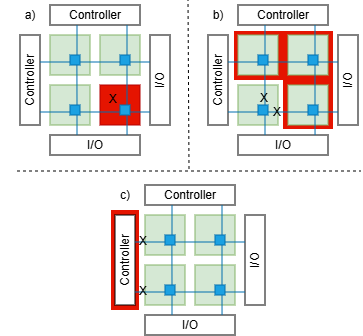
\includegraphics[width=0.95\linewidth]{body_chapters/chap_1/figs/2x2NoCFailure.png}
      \caption[CMP Failure Modes]{4-core CMP with a 2D mesh NoC interconnect. (a) Core failure due to wearout. (b) Router failure due to wearout. (c) Link failure due to wearout.}
      \label{fig:NoC_failure_modes}
  \end{center}
\end{figure}

Wearout in interconnects is particularly concerning because, unlike cores, which can often tolerate failures through redundancy or task remapping, failures in the interconnect are far more critical. As illustrated in Figure \ref{fig:NoC_failure_modes}, while a core failure (Fig. \ref{fig:NoC_failure_modes}a) may degrade performance, router (Fig. \ref{fig:NoC_failure_modes}b) or link failures (Fig. \ref{fig:NoC_failure_modes}c) can disrupt connectivity, partition the network, and render large portions of the system unusable.

Conventional routing algorithms, such as dimension-order routing (DOR), are oblivious to these effects. Their deterministic nature leads to uneven traffic distribution, with central routers and links experiencing consistently higher utilization. This imbalance translates directly into accelerated aging of specific components, effectively reducing the lifetime of the entire network. Prior work on NoC reliability has largely focused on fault-tolerant routing, where the objective is to maintain connectivity in the presence of permanent faults. These approaches are inherently reactive, requiring fault detection and reconfiguration after failures occur \cite{Adnan2025} \cite{Samala2020} \cite{Samala2022}. In contrast, aging-aware routing aims to delay the onset of such failures by controlling how traffic is distributed over time. This class of routing algorithms is fundamentally adaptive: routing decisions are influenced by dynamic metrics such as utilization, temperature, and accumulated wear, with the goal of balancing stress across the network and extending system lifetime.

Existing aging-aware routing techniques typically rely on explicit modeling of path reliability, combining metrics such as EM- and HCI-induced mean time to failure (MTTF) across candidate routes. While effective, these approaches often require global visibility of network state and repeated path evaluation, resulting in significant computational and storage overhead. Furthermore, their reliance on fixed cost functions and heuristics limits their ability to adapt to changing traffic patterns and evolving wear conditions over long execution periods \cite{Clotho2015} \cite{AROMa2018}.

\section{Problem Statement}

Current NoC routing algorithms do not account for long-term aging effects, leading to uneven wear and premature failure of critical components. Existing aging-aware approaches attempt to address this issue but often depend on "piggybacking" global information and fixed heuristics, making them difficult to scale and adapt to dynamic conditions.

This work focuses on developing a routing strategy that can adapt to changing network conditions while remaining lightweight and scalable, with the goal of improving overall system lifetime without significantly impacting performance.

\section{Scope of Research}

This thesis proposes a wear-aware routing approach based on linear approximate reinforcement learning. Instead of explicitly computing path reliability metrics, the routing policy is learned through interaction with the network, allowing the system to implicitly capture the relationship between traffic patterns and aging effects.

The key contributions of this work are:
\begin{itemize}
    \item A reinforcement learning-based aging-aware routing algorithm
    \item Integration of a linear function approximation model that enables scalability and low-overhead implementation at each router
    \item Integration of a deadlock-free adaptive routing design using escape virtual channels
    \item Implementation in the gem5 Garnet NoC simulator and evaluation demonstrating improved lifetime metrics
\end{itemize}
\chapter{Literature Review}

\section{Introduction to Routing Algorithms in NoCs}

Routing determines how packets travel through a Network-on-Chip from their source to their destination. In a typical 2D mesh NoC, each router forwards packets according to the routing algorithm implemented in its routing unit, with the overall goal of minimizing latency, sustaining throughput, and avoiding congestion and deadlock. NoC routing algorithms are broadly categorized as static or adaptive. Static routing uses fixed, predetermined paths independent of runtime conditions. Deterministic XY routing is the standard example, where packets are routed first in the X direction and then in the Y direction. Although this approach is simple and low cost, it does not react to traffic imbalance or failures, and can therefore create bottlenecks and underutilize alternative paths \cite{AROMa2018}.

Adaptive routing addresses this limitation by selecting routes based on the current network state, such as congestion levels, fault status, or buffer availability. These routing decisions may rely on local information, global information, or a hybrid of both, depending on the algorithm design. For this work, we are interested in adaptive routing only, which is best understood through the taxonomy proposed in the recent survey of 2D NoC routing \cite{Kondoth2026}, which divides adaptive approaches into reactive, proactive, and application-specific classes. Reactive routing responds to conditions that already exist in the network, while proactive routing attempts to prevent future degradation by anticipating harmful operating conditions.

Within reactive adaptation, one important class is fault-tolerant routing, whose objective is to preserve packet delivery by rerouting traffic around failed routers or links. Within proactive adaptation, one important class is aging-aware routing, which aims to reduce long-term wear by steering traffic away from components experiencing higher stress. In other words, fault-tolerant routing responds after faults occur, whereas aging-aware routing attempts to delay those faults by controlling the accumulation of wear over time \cite{Kondoth2026}. This work focuses on extending NoC lifetime as opposed to merely recovering from failure. The remainder of this literature review concentrates on adaptive routing methods in these two categories, with particular emphasis on aging-aware routing.

\section{Fault-Tolerant Routing Algorithm in NoC}

Fault-tolerant routing is concerned with maintaining communication in the presence of faulty routers or links. Its primary objective is to minimize packet loss and maximize successful packet delivery by rerouting traffic around failed components, while keeping latency and throughput within acceptable limits.

A simple approach is the dynamic XY-YX fault-tolerant routing algorithm \cite{An2021}, which switches from XY routing to YX routing when faults are encountered. However, the method is fundamentally constrained by a small set of predefined routing responses. Once faults create more complex blockage patterns, the algorithm cannot reason beyond the fixed XY/YX alternatives. Similar approaches are represented by logic- and rule-based fault-tolerant routing schemes summarized in the survey \cite{Kondoth2026}, such as FTMR, RAFT, Hermes, and related fault-ring or contour-based methods. These approaches identify faulty regions, classify unusable nodes, or maintain local fault information to bypass failed components. The drawback of these methods is that they depend on explicit fault modeling, packet-header updates, or region management logic, all of which add control overhead and can still lead to suboptimal paths when network conditions become more complex.

Recent work has therefore explored reinforcement learning (RL) as a way to make fault-tolerant routing more adaptive. In \cite{Jagadheesh2020}, routing is modeled as a Markov Decision Process and solved using Q-learning, with routers treated as states and routing decisions as actions. The proposed method is shown to find optimal paths in the presence of both router and link faults. On average, the paper reports about 19\% more delivered packets under link faults and 11\% more delivered packets under router faults. However, it relies on a large Q-table that grows with the number of routers and possible fault conditions, which can lead to high memory overhead. This limitation is addressed more directly in \cite{Samala2020}. This work extends the earlier RL-based mesh routing approach using decentralized multi-agent reinforcement learning and a two-level Q-table. The goal is to reduce the storage cost and stale-value issues associated with large flat Q-tables, while still learning effective fault-tolerant policies. More recent work \cite{LARE2023} shows that RL can improve network performance by learning better flit rerouting behavior.

\section{Aging-Aware Routing Algorithm}

Aging-aware routing aims to extend NoC lifetime by steering traffic away from components that are aging faster due to stress, temperature, and process variation. Unlike fault-tolerant routing, which reacts after failures occur, aging-aware routing attempts to delay failure by reducing the uneven accumulation of wear across routers and links. As the survey notes \cite{Kondoth2026}, the main evaluation metric in this class of work is typically MTTF, since the central objective is long-term reliability rather than immediate fault recovery.

One of the most influential works in this area is Clotho \cite{Clotho2015}, which frames wear-aware routing as a path-selection problem based on the lifetime of candidate routes. Clotho models both EM and HCI, while also incorporating temperature and process variation. Using these inputs, it computes a path metric over minimal routes and directs traffic toward paths with higher relative lifetime. Under PARSEC workloads, Clotho reports average MTTF improvements of 66\% for EM and 8\% for HCI over deterministic routing. However, Clotho relies on explicit path evaluation and "piggybacking" network lifetime information across the network, which introduces computational and memory overhead, and limits scalability.

A different line of work focuses on combining aging mitigation with performance control. Bhardwaj et al. \cite{Bhardwaj2012} introduces the Traffic Threshold per Epoch (TTpE) metric, which limits how much traffic a stressed router or link should accept during a given runtime interval. Its routing algorithm chooses paths that are both less stressed and less congested, and can insert recovery cycles once a component reaches its threshold. Experimentally, the paper reports reductions of 13\% in network latency, 12.17\% in EDPPF, and a 10.4\% performance improvement over its comparison scheme. However, this method relies on precomputed lifetime models and static thresholds, which may not adapt well to changing runtime conditions or workloads.

Another important direction is online monitoring-based aging awareness. In \cite{Ghaderi2017}, Ghaderi et al. propose a Centralized Aging Table (CAT) that maps observed router activity to aging degradation. Their method monitors the number of flits and residence time within routers, then periodically updates routing to avoid highly aged routers by selecting among shortest paths. Using gem5, it reports average improvements of 39\% in maximum-aged router degradation and 52\% in aging imbalance compared to XY routing, while introducing negligible overhead in latency and EDP. This idea is extended further in AROMa \cite{AROMa2018}, which targets 3D NoCs. It uses a Distributed Centralized Aging Table (D-CAT), with a separate table per layer, and periodically swaps among k-best shortest paths to avoid highly aged routers and allow BTI recovery. Compared to non-aging-aware routing, it improves maximum age by about 33-34\% and age imbalance by 61-72\%, with the 3D case showing especially strong gains. However, both CAT and D-CAT rely on explicit aging tables and synchronizing aging information across the network, which can introduce memory overhead and limit scalability as the NoC size increases.

\section{Gaps in Prior Studies}

Prior studies on NoC routing algorithms has made significant progress in both fault-tolerant and aging-aware routing. However, there are still important gaps that this thesis aims to address. First, many aging-aware routing methods rely on explicit aging models or tables that require global state and synchronization, which can limit scalability and adaptability to changing conditions. Second, while RL-based fault-tolerant routing has shown promise, it has not been widely applied to aging-aware routing, which also requires dynamic adaptation to runtime conditions. The main trade-off across the literature is between model fidelity and implementation overhead. To this end, this work proposes to fill these gaps by developing a wear-aware routing algorithm that leverages linear approximate reinforcement learning to adaptively steer traffic away from stressed components without relying on explicit aging tables or models, while also maintaining acceptable network performance.
\chapter{Aging-Aware Routing Algorithm System Design}

This section presents the system-level modeling framework and design choices used to enable reliability-aware routing in the NoC. The proposed approach integrates dynamic temperature variation, process variation, and aging models for EM and HCI directly into the routing decision process. These models are based on prior work in \cite{Clotho2015} and are combined with a reinforcement learning-based routing policy inspired by LARE \cite{LARE2023}.

Although other aging mechanisms, such as Bias Temperature Instability (BTI), also affect CMOS devices, they are not considered here. As discussed in \cite{Clotho2015}, BTI degradation is primarily associated with underutilized circuits and can be mitigated using techniques such as \textit{Use it or Lose it} \cite{Kim2013}. In contrast, EM and HCI are driven by switching activity and temperature, making them closely tied to traffic patterns and more appropriate for routing-level optimization.

Unlike conventional routing algorithms that optimize only performance metrics such as latency and throughput, this framework incorporates device-level reliability into routing decisions. Temperature and utilization are modeled as dynamic runtime inputs, while process variation is treated as a static parameter determined during initialization.

\section{Dynamic Temperature Variation}

Temperature is one of the primary factors governing the rate of both EM and HCI induced aging, and is therefore modeled explicitly as a dynamic runtime parameter. In a CMP, temperature is not spatially uniform. Instead, it varies across the die due to non-uniform activity in the processing and memory resources, which arises from application mapping, workload imbalance, and differences in instruction behavior. Following the modeling approach used in Clotho \cite{Clotho2015}, the chip is partitioned into an $n \times n$ grid of equal-area tiles. Each tile represents a thermal region containing one processing core, its associated cache resources, and the locally connected router with its nearest-neighbor bidirectional links. Within each tile, temperature is assumed to be uniform, while different tiles may exhibit different temperatures. This assumption is justified by the observation that the NoC contributes only a relatively small fraction of the total chip power budget, and that this power is spatially distributed across the die rather than concentrated in a small number of locations. Consequently, the dominant source of thermal variation is taken to be the computational activity of the processing elements, while the routers are treated as thermally coupled to the tiles that contain them \cite{Clotho2015}.

\begin{figure}[ht]
    \centering
    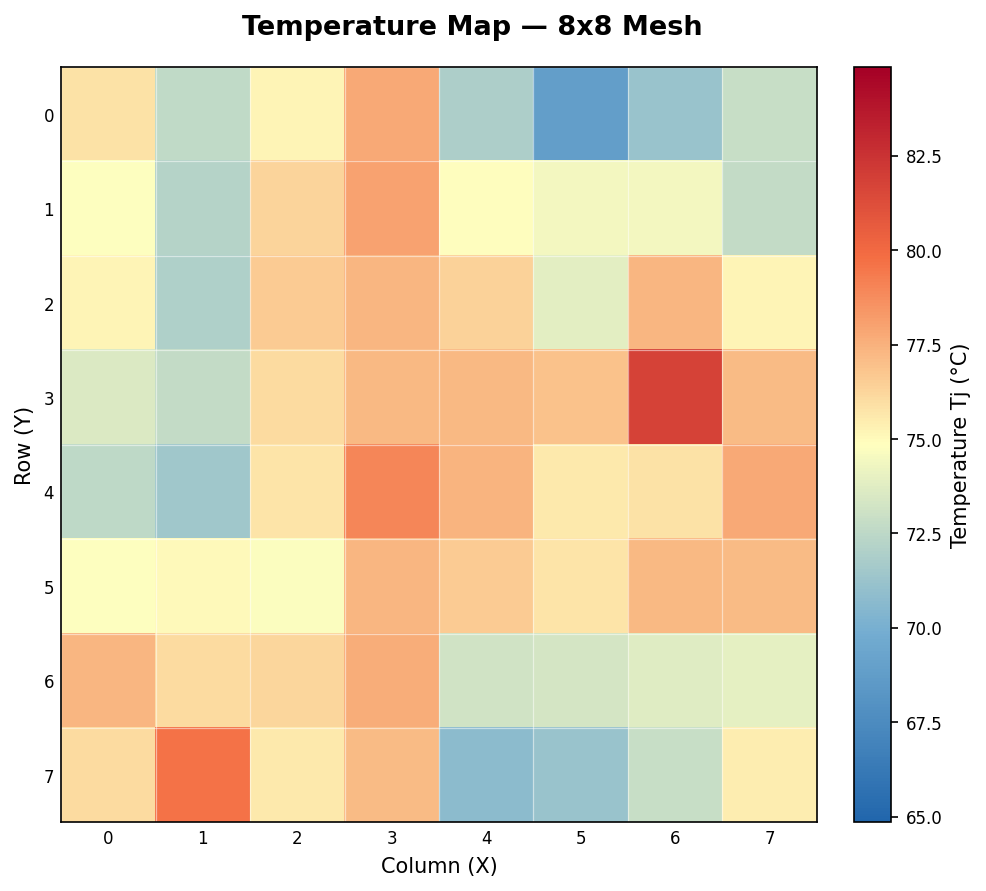
\includegraphics[width=0.95\linewidth]{body_chapters/chap_3/figs/temperature_map.png}
    \caption[Per-router temperature map]{Example spatial mapping of temperature across the NoC. The map reflects the combination of spatially correlated thermal variation.}
    \label{fig:temp_maps}
\end{figure}

Temperature is modeled as a slowly varying parameter rather than as a quantity that changes every cycle. In Clotho, the absolute values of the temperature map are updated every $10^7$ cycles in order to emulate the gradually changing thermal behavior of a running CMP, consistent with prior observations that on-chip temperature sensing and thermal evolution occur over millisecond-scale intervals rather than cycle-by-cycle timescales \cite{Clotho2015}. The same assumption is adopted here. Accordingly, the temperature map is periodically refreshed every $10^7$ cycles, allowing the routing algorithm to respond to long-term changes in the thermal profile without introducing unnecessary per-cycle thermal recomputation. The temperature assigned to each tile is generated as part of a spatial temperature map spanning the range of 65$^\circ$C to 85$^\circ$C, consistent with the range used in Clotho \cite{Clotho2015}. In implementation, these values are generated using a random but spatially correlated distribution so that neighboring tiles tend to exhibit similar thermal behavior. Figure \ref{fig:temp_maps} illustrates an example of such a temperature map. This per-tile temperature information is then used directly by the EM and HCI aging models. Since both failure mechanisms accelerate at higher temperatures, tiles operating at elevated temperature accumulate wear more rapidly than cooler tiles under otherwise similar activity conditions.

\section{Process Variation}

Process variation (PV) arises from fabrication-time imprecision and results in deviations of transistor parameters from their nominal values. As CMOS technology scales, these variations become more pronounced and introduce spatial non-uniformity in device characteristics across the chip. In the context of NoC reliability, PV plays an important role in modulating aging behavior, particularly for HCI, where transistor-level characteristics directly influence degradation rates \cite{Clotho2015}.

Following the Clotho model, PV is captured by considering variations in two key transistor parameters: the threshold voltage ($V_{th}$) and the effective gate length ($L_{eff}$). For each router, these parameters are modeled as:
\begin{equation}
V_{th} = V_{th0} + \Delta V_{th}, \quad V_{th0} = 179\ \text{mV}
\end{equation}
\begin{equation}
L_{eff} = L_{eff0} + \Delta L_{eff}, \quad L_{eff0} = 14.4\ \text{nm}
\end{equation}

The deviations $\Delta V_{th}$ and $\Delta L_{eff}$ are composed of two independent components:
\begin{equation}
\Delta V_{th} = \Delta V_{th,rand} + \Delta V_{th,sys}
\end{equation}
\begin{equation}
\Delta L_{eff} = \Delta L_{eff,rand} + \Delta L_{eff,sys}
\end{equation}

Systematic variation represents spatially correlated deviations caused by layout-dependent and process-wide effects. Neighboring regions of the chip tend to exhibit similar variation values. As in Clotho, systematic variation is modeled using a multivariate normal distribution with a spherical spatial correlation structure. The correlation between two regions depends only on their Euclidean distance $r$:
\begin{equation}
\rho(r) =
\begin{cases}
1 - \frac{3r}{2\phi} + \frac{r^3}{2\phi^3}, & r \leq \phi \\
0, & r > \phi
\end{cases}
\end{equation}
where $\phi$ represents the correlation range expressed as a fraction of the die length. In this work, $\phi = 0.5$, meaning that routers separated by more than half the die are effectively uncorrelated. Within a single region, variation is fully correlated ($\rho(0) = 1$), while distant regions exhibit no correlation \cite{Clotho2015}.

Random variation, in contrast, is uncorrelated and occurs at a much finer granularity, reflecting device-level fluctuations such as dopant variation. Both random and systematic components are assumed to follow normal distributions with zero mean. Since these components are independent, the total variation also follows a normal distribution with:
\begin{equation}
\sigma_{total} = \sqrt{\sigma_{rand}^2 + \sigma_{sys}^2}
\end{equation}

The parameter values used in this work are taken directly from Clotho and are summarized as follows:
\begin{itemize}
    \item For $V_{th}$: $\sigma_{rand} = 6.3\%$, $\sigma_{sys} = 6.3\%$
    \item For $L_{eff}$: $\sigma_{rand} = 3.2\%$, $\sigma_{sys} = 3.2\%$
    \item Correlation range: $\phi = 0.5$
\end{itemize}

Process variation is treated as a static property determined at fabrication time. Accordingly, the values of $V_{th}$ and $L_{eff}$ are generated once during initialization and remain constant throughout execution. In the implemented model, each router is assigned a fixed pair of $(V_{th}, L_{eff})$ values, which are stored and used throughout the simulation.

To visualize the spatial effect of process variation across the NoC, Figure \ref{fig:pv_maps} illustrates example per-router maps of the generated threshold voltage and effective gate length values. Since the systematic component is spatially correlated, neighboring routers tend to exhibit similar deviations, producing smooth regional variation rather than entirely independent fluctuations. The random component is then superimposed locally, yielding the final per-router values used in the model. Since process variation is not uniform across the chip, different routers may begin operation with different intrinsic susceptibility to HCI-induced degradation.

\begin{figure}[ht]
    \centering
    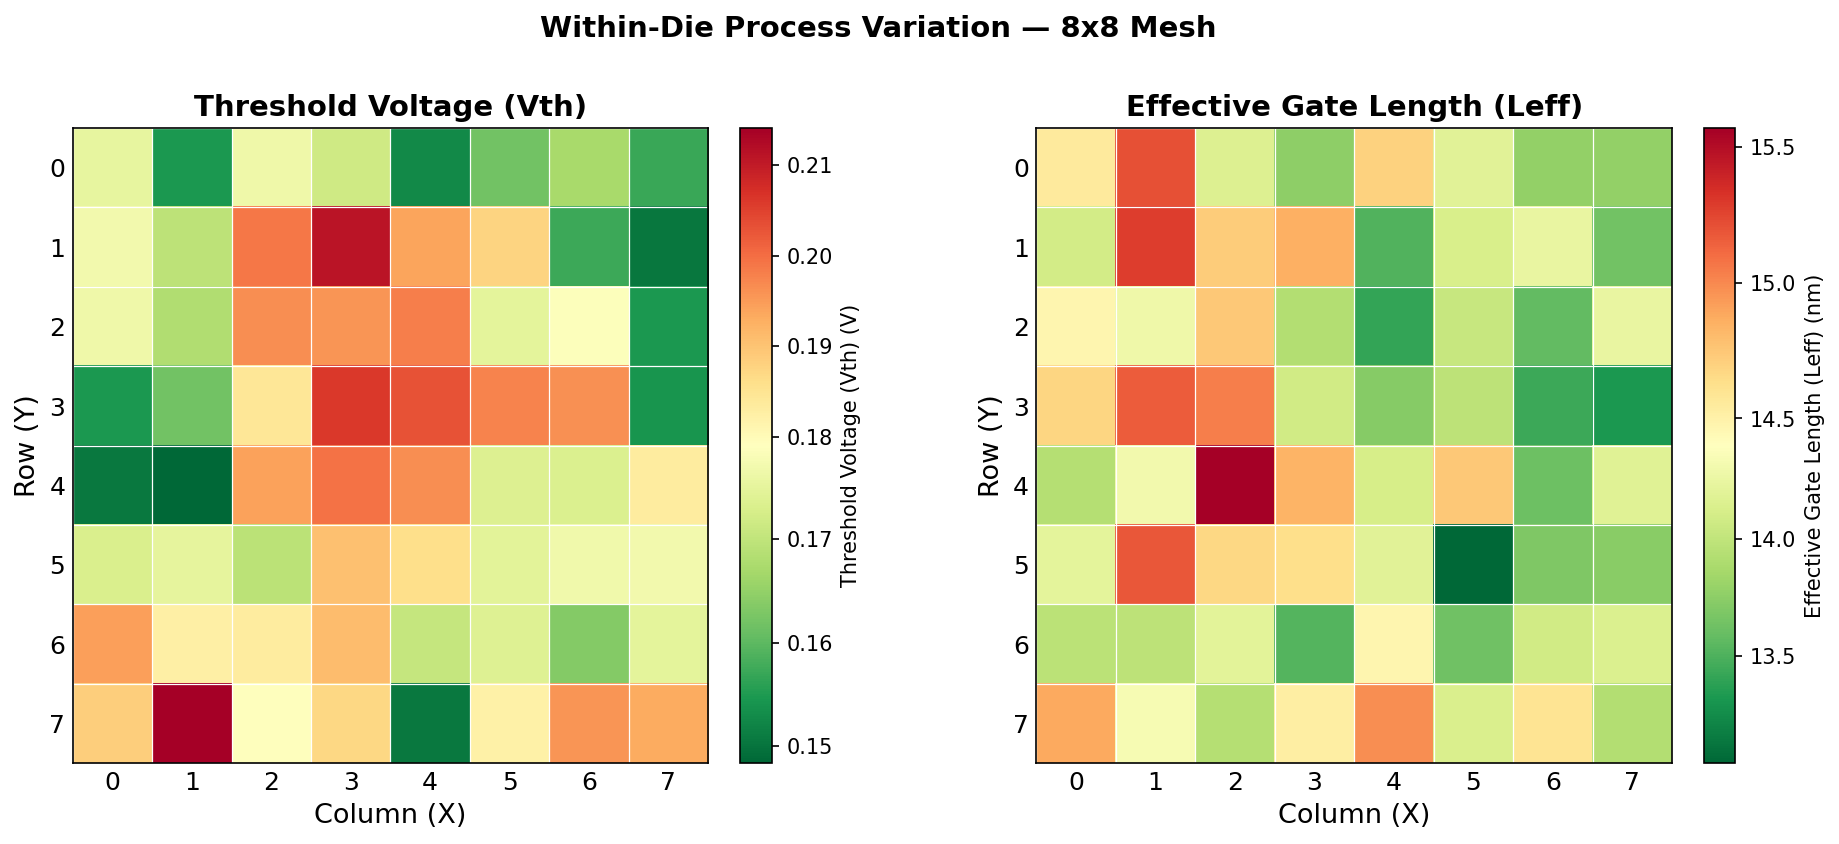
\includegraphics[width=1\linewidth]{body_chapters/chap_3/figs/process_variation_map.png}
    \caption[Per-router process variation maps]{Example spatial mapping of process variation across the NoC: (left) threshold voltage, $V_{th0} + \Delta V_{th}$, and (right) effective gate length, $L_{eff0} + \Delta L_{eff}$, for all routers in the mesh. The maps reflect the combination of spatially correlated systematic variation and uncorrelated random variation applied at initialization.}
    \label{fig:pv_maps}
\end{figure}

The resulting per-router values of $V_{th}$ and $L_{eff}$ are subsequently used to compute the substrate current ($I_{sub}$), which serves as an intermediate quantity in the HCI aging model. Since PV is static and all other parameters involved in this computation are technology constants, $I_{sub}$ can be precomputed once at initialization. The computation proceeds as follows:

\begin{equation}
V_{dsat} = \frac{(V_{gs} - V_{th}) \cdot L_{eff} \cdot E_{cr}}{(V_{gs} - V_{th}) + L_{eff} \cdot E_{cr}}
\end{equation}

where $V_{gs}$ is the gate-to-source voltage, $V_{th}$ is the threshold voltage, and $E_{cr}$ denotes the critical electric field associated with velocity saturation.

\begin{equation}
E_m = \frac{V_{ds} - V_{dsat}}{\sqrt{3 t_{ox} x_j}}
\end{equation}

where $V_{ds}$ denotes the drain-to-source voltage and $V_{dsat}$ corresponds to the voltage at the channel pinch-off point. The term $\sqrt{3 t_{ox} x_j}$ represents a characteristic length associated with the effective thickness of the pinch-off region in the transistor channel. For typical CMOS technologies, this length falls within the range $\sqrt{100\ \text{nm}}$ to $\sqrt{300\ \text{nm}}$.

\begin{equation}
I_{sub} = C_2 \cdot I_{ds} \cdot \exp\left(\frac{-\phi_i}{q \lambda_e E_m}\right)
\end{equation}

where $C_2$ is a proportionality constant, $I_{ds}$ is the drain current, $\phi_i$ denotes the minimum energy required for a hot electron to initiate impact ionization, $q$ is the elementary charge, $\lambda_e$ is the mean free path of hot electrons, and $E_m$ is the electric field in the channel.

All parameters other than $V_{th}$ and $L_{eff}$ are treated as technology-dependent constants and are fixed based on values reported in prior work. The resulting $I_{sub}$ value is stored as a single scalar per router, eliminating the need for repeated evaluation of the above expressions during runtime. The precomputed $I_{sub}$ is later used in the HCI aging model to determine degradation rates as a function of switching activity and temperature.

\section{Aging Models}

\subsubsection{Electromigration (EM)}

Electromigration (EM) is a wearout mechanism in which momentum transfer from conducting electrons causes gradual displacement of metal ions in interconnect wires. Under sustained high current density, this ion migration leads to the formation of voids and hillocks, eventually resulting in open- or short-circuit failures. As technology scales and interconnect dimensions shrink, current densities increase, making EM a critical reliability concern in modern NoCs \cite{Clotho2015}.

The lifetime of an interconnect under EM stress is commonly modeled using Black's equation:
\begin{equation}
MTTF_{EM} = A_{EM} J^{-n} \exp\left(\frac{E_{a,EM}}{kT}\right)
\end{equation}
where $J$ is the current density, $n$ is an empirical exponent (typically close to 2), $E_{a,EM}$ is the activation energy, $T$ is temperature, and $k$ is Boltzman's constant.

In NoC interconnects, current density is closely related to switching activity. As traffic increases, links are exercised more frequently, leading to a higher rate of current flow through the interconnect. Long router-to-router links tend to carry a larger share of traffic and exhibit higher effective current density compared to shorter intra-router wires. As a result, these links are more susceptible to electromigration-induced degradation.

Following \cite{Clotho2015}, current density is expressed in terms of link switching activity:
\begin{equation}
J \propto \alpha_{link}
\end{equation}

Substituting this relationship into Black's equation yields a simplified proportional model:
\begin{equation}
MTTF_{EM}(\alpha_{link}, T) \propto \alpha_{link}^{-2} \cdot \exp\left(\frac{E_{a,EM}}{kT}\right)
\end{equation}

The switching activity $\alpha_{link}$ is derived from link utilization:
\begin{equation}
\alpha_{link} = 0.5 \times U_{link}
\end{equation}
which assumes random data patterns, where each bit has a 50\% probability of switching.

In this work, EM is modeled at the granularity of individual links. A proportional MTTF value is computed for each link based on its runtime utilization and temperature. These values are updated periodically as network conditions evolve.

A key characteristic of this model is its quadratic dependence on switching activity. As a result, EM is highly sensitive to traffic distribution. Even modest reductions in link utilization can produce significant improvements in lifetime. This makes EM particularly responsive to routing-level load balancing, where redistributing traffic away from heavily utilized links can substantially reduce localized wear.

\subsubsection{Hot-Carrier Injection (HCI)}

Hot-carrier injection (HCI) is a transistor-level aging mechanism caused by high-energy carriers that become trapped in the gate oxide during switching. Over time, this leads to a gradual increase in threshold voltage ($V_{th}$), which slows transistor switching speed and degrades circuit performance. In NoC routers, this degradation is most critical along timing-critical paths, where increased delay can eventually result in timing violations and system failure \cite{Clotho2015}.

The lifetime of a device under HCI stress can be expressed as:
\begin{equation}
MTTF_{HCI}^{DC} = A_{HCI} (I_{sub})^{-N} \exp\left(\frac{E_{a,HCI}}{kT}\right)
\end{equation}
where $I_{sub}$ is the substrate current during stress, $N$ is an empirical exponent (approximately 1.5), and $E_{a,HCI}$ is the activation energy.

Since HCI degradation occurs during switching events, its impact under dynamic operation is proportional to switching activity. Incorporating this effect yields:
\begin{equation}
MTTF_{HCI}^{AC}(\alpha_{router}, T) \propto \frac{(I_{sub})^{-N}}{\alpha_{router}} \cdot \exp\left(\frac{E_{a,HCI}}{kT}\right)
\end{equation}

Here, $\alpha_{router}$ represents the switching activity along the router’s critical path. Based on empirical observations in \cite{Clotho2015}, this activity is related to router utilization by:
\begin{equation}
\alpha_{router} = 0.1 \times U_{router}
\end{equation}
reflecting that only a subset of flits (primarily header flits) exercise the critical path.

Unlike EM, HCI is strongly influenced by process variation. Variations in threshold voltage ($V_{th}$) and effective gate length ($L_{eff}$) affect the substrate current $I_{sub}$, which in turn determines degradation rate. As described in the previous section, $I_{sub}$ is computed per router as a function of these parameters and treated as a static quantity throughout execution.

Combining these effects yields the final HCI model used in this work:
\begin{equation}
MTTF_{HCI,PV} \propto \frac{(I_{sub}(V_{th}, L_{eff}))^{-N}}{\alpha_{router}} \cdot \exp\left(\frac{E_{a,HCI}}{kT}\right)
\end{equation}

This model captures both dynamic and static sources of degradation. The switching activity and temperature introduce time-varying stress, while process variation establishes a fixed baseline reliability for each router. As a result, routers with unfavorable $(V_{th}, L_{eff})$ values begin operation with reduced timing margin and are inherently more vulnerable to HCI-induced degradation.

Compared to EM, HCI exhibits a weaker dependence on switching activity due to its linear relationship with $\alpha_{router}$. Consequently, while traffic redistribution can still improve HCI lifetime, its impact is less pronounced than in the case of EM.

\subsubsection{Utilization of Lifetime Models}

The EM and HCI models described above are used to guide routing decisions and evaluate system reliability. During routing, the MTTF of candidate next-hop links and routers is computed using current utilization and temperature values. These MTTF estimates are normalized relative to the network state and used to define the reward signal for the reinforcement learning policy. Routing decisions are therefore biased toward paths that traverse components with higher estimated lifetime.

Throughout simulation, MTTF values are updated periodically as utilization statistics and temperature maps are refreshed. This enables the system to track the evolution of wear across all network components under dynamic traffic conditions. At the end of simulation, the final MTTF values of all routers and links are collected. The system lifetime is defined by the most degraded component, reflecting the fact that failure of a single critical link or router can render the network unusable.

To compare routing algorithms, the acceleration factor (AF) is used as a relative lifetime metric:
\begin{equation}
AF_{EM} = \frac{MTTF_{EM}|_{RL}}{MTTF_{EM}|_{DOR}}, 
\quad
AF_{HCI} = \frac{MTTF_{HCI,PV}|_{RL}}{MTTF_{HCI,PV}|_{DOR}}
\end{equation}

Since both configurations share identical process variation and technology parameters, unknown constants and the precomputed $I_{sub}$ cancel out in the ratio. As a result, the acceleration factor depends only on runtime variables such as utilization and temperature.

\section{Reinforcement Learning-Based Routing Policy}

Reinforcement learning (RL) is a learning framework in which an agent interacts with an environment to learn a policy that maximizes long-term cumulative reward. At each decision step, the agent observes the current state $s$, selects an action $a$, and receives a reward $r$ based on the outcome of that action. The system then transitions to a new state $s'$, and the process repeats. Over time, the agent improves its decision-making by learning from these interactions. Figure~\ref{fig:RL_framework} illustrates this agent–environment interaction model.

\begin{figure}[ht]
  \centering
  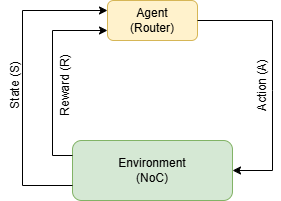
\includegraphics[width=0.7\linewidth]{body_chapters/chap_3/figs/RL.png}
  \caption[Reinforcement Learning Framework]{Agent–environment interaction in reinforcement learning.}
  \label{fig:RL_framework}
\end{figure}

In this work, we adopt Q-learning, a value-based RL method. Q-learning estimates the expected cumulative reward of taking an action $a$ in a state $s$, represented by the Q-value function $Q(s,a)$. The optimal policy is obtained by selecting actions that maximize this value.

The Q-values are updated iteratively using the Bellman equation:

\begin{equation}
Q(s,a) \leftarrow Q(s,a) + \alpha \left[ r + \gamma \max_{a'} Q(s',a') - Q(s,a) \right]
\end{equation}

where $\alpha$ is the learning rate and $\gamma$ is the discount factor. The term inside the brackets is the temporal-difference (TD) error, which measures how well the current estimate matches observed outcomes.

In the context of NoCs, routing decisions can be formulated as a sequential decision-making problem, where each router selects the next-hop direction for a packet based on local network conditions. Each router is modeled as an independent RL agent, and routing corresponds to selecting an action that maximizes long-term reward. Direct application of tabular Q-learning, however, is impractical in NoCs due to the large state-action space, which grows rapidly with network size. This leads to excessive storage requirements and slow convergence, commonly referred to as the curse of dimensionality. To address this limitation, this work adopts a linear function approximation approach inspired by LARE \cite{LARE2023}, where Q-values are represented using a compact feature-based model instead of a lookup table.

\subsubsection{State Representation}

Routing decisions are made at each router when multiple minimal paths are available. Instead of representing the state explicitly, each state-action pair $(s,a)$ is encoded using a feature vector $\phi(s,a)$:

\begin{equation}
\phi(s,a) = [f_0, f_1, f_2, f_3, f_4, f_5, f_6, f_7, f_8]
\end{equation}

where:
\begin{itemize}
    \item $f_0$: Bias term (constant 1)
    \item $f_1$: Destination router ID
    \item $f_2$: Current router ID
    \item $f_3$: Distance traveled in hops from source to current router
    \item $f_4$: Remaining distance to destination
    \item $f_5$: EM MTTF of candidate link
    \item $f_6$: HCI MTTF of candidate router
    \item $f_7$: Output port congestion level
    \item $f_8$: Encoded input port direction
\end{itemize}

This representation allows the agent to incorporate both performance related and reliability related information into routing decisions.

\subsubsection{Q-Value Function}

To reduce hardware overhead, the Q-value is approximated using a linear function:

\begin{equation}
Q(s,a) = \theta_0 \cdot f_0 + \theta_1 \cdot f_1 + \theta_2 \cdot f_2 + \theta_3 \cdot f_3 + \theta_4 \cdot f_4 + \theta_5 \cdot f_5 + \theta_6 \cdot f_6 + \theta_7 \cdot f_7 + \theta_8 \cdot f_8
\end{equation}

where $f_i$ represents the $i$-th feature in the state-action vector, and $\theta_i$ is the corresponding learned coefficient. Each coefficient captures the contribution of its feature toward the estimated long-term reward.

This approach eliminates the need to store a full Q-table, reducing memory requirements and enabling scalable implementation at the router level, while still allowing the model to capture relationships between features and long-term reward.

\subsubsection{Action Selection Policy}

An $\epsilon$-greedy policy is used to balance exploration and exploitation:

\begin{equation}
a =
\begin{cases}
\text{random action}, & \text{with probability } \epsilon \\
\arg\max_a Q(s,a), & \text{otherwise}
\end{cases}
\end{equation}

The action space consists of minimal routing directions (e.g., horizontal and vertical moves in a mesh topology).

\subsubsection{Reward Function}

The reward function is designed to jointly capture reliability and performance objectives. It combines normalized aging metrics with congestion information:

\begin{equation}
R = 0.7 \cdot \text{MTTF}_{score} - 0.3 \cdot \text{cong}_{norm}
\end{equation}

The reliability component is defined as:
\begin{equation}
\text{MTTF}_{score} = C_{EM} \cdot EM_{norm} + C_{HCI} \cdot HCI_{norm}
\end{equation}

The EM and HCI values are normalized across candidate actions:
\begin{equation}
EM_{norm} = \frac{MTTF_{EM}}{\max(MTTF_{EM}^{(h)}, MTTF_{EM}^{(v)})}
\end{equation}

\begin{equation}
HCI_{norm} = \frac{MTTF_{HCI}}{\max(MTTF_{HCI}^{(h)}, MTTF_{HCI}^{(v)})}
\end{equation}

where the superscripts $(h)$ and $(v)$ denote the horizontal and vertical candidate next hops, respectively.

To dynamically emphasize the more critical aging mechanism, adaptive weights are computed using:

\begin{equation}
C(x) =
\frac{\exp\left(8 \cdot \frac{x - x_{min}}{x_{max} - x_{min}}\right) - \exp(-8)}
{1 - \exp(-8)}
\end{equation}

where $x \in \{MTTF_{EM}, MTTF_{HCI}\}$, and $x_{max}$ and $x_{min}$ are the maximum and minimum values among candidate actions. The weights are then defined as:

\begin{equation}
C_{EM} = C(MTTF_{EM}), \quad C_{HCI} = C(MTTF_{HCI})
\end{equation}

The congestion term reflects the load on the output port:
\begin{itemize}
    \item Low congestion: $0$
    \item Medium congestion: $0.5$
    \item High congestion: $1.0$
\end{itemize}

This formulation encourages the routing policy to prefer paths that both reduce congestion and avoid highly stressed components.

\subsubsection{Update Rule}

The parameter vector $\theta$ is updated using temporal-difference learning. First, the TD error is computed:

\begin{equation}
\delta = R + \gamma \max_{a'} Q(s', a') - Q(s,a)
\end{equation}

The parameters are then updated as:

\begin{equation}
\theta \leftarrow \theta + \alpha \cdot \delta \cdot \phi(s,a)
\end{equation}

This update adjusts the model parameters in the direction that reduces the discrepancy between predicted and observed rewards, allowing the routing policy to improve over time.

\section{Deadlock Avoidance}

Adaptive routing algorithms, including the proposed RL-based routing policy, do not inherently guarantee deadlock freedom \cite{LARE2023}. Since routing decisions are made dynamically based on network conditions, packets may acquire resources in different orders, potentially leading to cyclic dependencies. To understand how deadlock arises and how it can be prevented, it is first necessary to examine the underlying router microarchitecture.

\subsubsection{Router Microarchitecture}

A typical NoC router employs virtual channel (VC) flow control to efficiently utilize network resources. As shown in Figure~\ref{fig:router_arch}, each router consists of input ports with associated buffers, a routing unit, a switch allocator, a crossbar, and output ports.

\begin{figure}[ht]
    \centering
    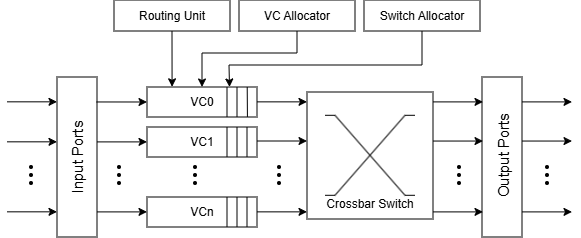
\includegraphics[width=0.95\linewidth]{body_chapters/chap_3/figs/router.png}
    \caption[NoC Router Microarchitecture]{Router microarchitecture based on virtual channel flow control.}
    \label{fig:router_arch}
\end{figure}

Incoming packets arrive at an input port and are stored in input buffers organized as multiple virtual channels. Each VC maintains a separate queue of flits, allowing multiple packets to share the same physical channel without blocking each other. When a packet reaches the head of a VC, the routing unit determines the set of candidate output ports based on the routing algorithm. The packet then requests access to a downstream VC at the next router. Once a downstream VC is successfully allocated, the packet competes for access to the crossbar through the switch allocator. If granted, the packet is forwarded through the crossbar to the selected output port and transmitted to the next router. This process repeats at each hop, resulting in a sequence of resource acquisitions: input VC, downstream VC, switch allocation, and output link traversal.

\subsubsection{Deadlock Formation}

The staged allocation of resources creates dependencies between packets across routers. A packet occupying a VC at one router may be blocked while waiting for a downstream VC at the next router. If that downstream VC is already occupied by another packet, the dependency extends further along the network. Deadlock occurs when a set of packets forms a cyclic dependency, where each packet holds a resource while waiting for another resource held by another packet in the cycle.

\begin{figure}[ht]
    \centering
    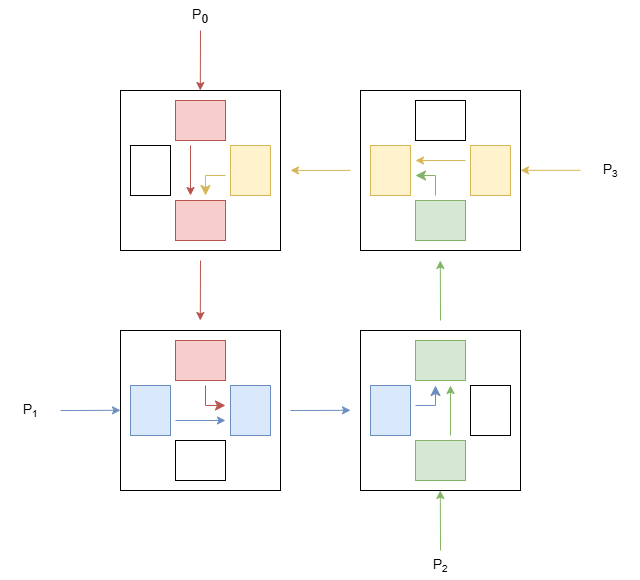
\includegraphics[width=0.95\linewidth]{body_chapters/chap_3/figs/deadlock.png}
    \caption[Deadlock Formation]{Example of cyclic resource dependency leading to deadlock in a mesh NoC.}
    \label{fig:deadlock_cycle}
\end{figure}

In a 2D mesh, such cycles can occur when packets routed in different directions occupy VCs in neighboring routers while waiting for each other's downstream resources, forming a closed loop. Since none of the packets can release their current resources until they acquire the next one, no forward progress is possible. This is illustrated in Figure~\ref{fig:deadlock_cycle}, where packets $P_0$, $P_1$, $P_2$, and $P_3$ form a cycle of dependencies across four routers. Each packet is waiting for a buffer in the downstream router that is currently being occupied by another packet in the cycle, resulting in a situation where no packet can proceed and the system is effectively stalled.

Adaptive routing increases the likelihood of such cycles because it allows packets to dynamically select different paths. Unlike deterministic routing, which enforces a strict ordering of channel acquisition, adaptive routing introduces flexibility that can lead to arbitrary dependency patterns and potential deadlock.

\subsubsection{Deadlock Avoidance Using Escape Virtual Channels}

To guarantee deadlock freedom, this work adopts an escape virtual channel mechanism based on Duato's theory \cite{Duato1993}. The key idea is to reserve a subset of network resources that follow a strictly deadlock-free routing function, ensuring that at least one acyclic path is always available.

In this implementation, one virtual channel (VC0) is designated as the escape channel and is restricted to deterministic dimension-order (XY) routing. Since XY routing enforces a strict ordering of channel acquisition and is provably deadlock-free, any packet assigned to this channel is guaranteed forward progress. All remaining virtual channels are allowed to use the RL-based adaptive routing policy. If a packet cannot safely proceed using adaptive routing, it can transition to the escape VC and continue using XY routing. This mechanism ensures that cyclic dependencies are avoided while preserving the flexibility of adaptive routing for the majority of traffic.

% \section{Tables}

% Tables can be placed with the \textbf{\textbackslash table} environment. The same instructions for the figures apply here; use the \textbf{\textbackslash label} command often

% \begin{center}
%   \begin{table}[h]
%     \centering
%     \begin{tabular}{l c l c}
%     \hline
%     Layer Type & Size & Activation & Regularization\\
%     \hline
%     Flatten& $30 \times 30 \times 3$ &ReLU & ---\\
%     Dense & 4096 & ReLU & 10\% Dropout\\
%     Dense & 2048 & ReLU & 10\% Dropout\\
%     Dense & 1024 & ReLU & 10\% Dropout\\
%     Dense & 1024 & ReLU & --- \\
%     Dense & 6 & Softmax & --- \\
%     \hline
%     \end{tabular}
%     \caption[Short Caption for List of Tables.]{Long caption to appear in the body of the text with the table.}
%     \label{tab:ModelArchitecture}
%   \end{table}
% \end{center}

\chapter{Evaluation}

\section{Simulation Setup}

All simulations are conducted using the gem5 Garnet cycle-accurate NoC simulator \cite{gem5} \cite{lowepower2020gem5simulatorversion200} in standalone synthetic traffic mode, without a full CPU or ISA model, to isolate network behavior. The network consists of 64 nodes arranged in an $8 \times 8$ 2D mesh topology. Each node acts as both a traffic source and destination, with packets injected according to configurable synthetic traffic patterns at a specified rate in packets per cycle per node.

The simulated clock frequency is 1 GHz. The router microarchitecture is an input-queued, virtual-channel router with credit-based flow control. Each router has a pipeline latency of 1 cycle and each link has a traversal latency of 1 cycle. The network supports three virtual networks per input port: two control virtual networks (vnets 0 and 1) and one data virtual network (vnet 2). Each virtual network contains 4 virtual channels. Control virtual channels have a buffer depth of 1 flit, while data virtual channels have a buffer depth of 4 flits. Control messages (vnets 0 and 1) consist of a single flit, whereas data messages (vnet 2) consist of 5 flits. The flit width is 128 bits (16 bytes).

The RL-based routing agent is trained over 50 million cycles, using uniform random traffic at an injection rate of 0.2 packets/cycle/node. The learned weight vectors are saved at the end of training run. The learning rate ($\alpha$), exploration rate ($\epsilon$), and discount factor ($\gamma$) are set to 0.01, 0.1, and 0.9, respectively.

For evaluation, the exploration rate is set to $\epsilon = 0$, resulting in a purely greedy policy with no further updates. Both the RL-based routing scheme and the DOR baseline are evaluated across a range of injection rates. Each configuration is simulated for 50 million cycles across multiple synthetic traffic patterns, including uniform random, neighbor, transpose, shuffle, bit reverse, and bit rotation.

The wearout state used in the RL reward is updated periodically during simulation. Link and router utilization are sampled every 1,000 cycles as a windowed average. The spatially correlated temperature map is regenerated every $10^7$ cycles. Process variation parameters ($\Delta V_{th}$, $\Delta L_{eff}$) are sampled once at initialization, ensuring identical per-router $I_{sub}$ values across both RL and DOR runs.

\section{Garnet Synthetic Traffic and Evaluation Metrics}

To evaluate the proposed routing approach under a wide range of network conditions, simulations are conducted using seven synthetic traffic patterns: uniform random, neighbor, transpose, tornado, shuffle, bit reverse, and bit rotation. These patterns generate diverse spatial load distributions, resulting in different stress profiles across routers and links and near 100\% network utilization.

Uniform random traffic selects destinations uniformly, producing a balanced load across the network. Neighbor traffic restricts communication to adjacent nodes. Transpose traffic maps each node at position $(i, j)$ to $(j, i)$. Tornado traffic sends packet from a node (i, j) in a NxM mesh to a destination node which is offset by roughly half the circumference of the mesh. Shuffle, bit reverse, and bit rotation are structured permutation patterns derived from bitwise transformations of node indices, which create asymmetric and pattern-dependent congestion across the network.

For each traffic pattern, injection rates are swept to capture both low-load and high-load regimes. For uniform random and neighbor traffic, injection rates range from 0.01 to 0.40 packets/cycle/node in increments of 0.03. For the remaining patterns, injection rates range from 0.01 to 0.20 in increments of 0.01. Each configuration is simulated for 50 million cycles.

The evaluation focuses on both performance and reliability metrics. Performance is characterized using average packet latency and throughput, while reliability is assessed using the AF derived from EM and HCI lifetime models. Together, these metrics provide a comprehensive view of the trade-offs between network efficiency and long-term wear.

\section{Results}

\subsubsection{Acceleration Factor}

To summarize the reliability improvements across traffic patterns, the mean Acceleration Factor (AF) for the weakest 10\% of components is presented using bar charts (Figures~\ref{fig:af_links_bar} and \ref{fig:af_routers_bar}). Detailed AF trends as a function of injection rate are provided in the appendix \ref{chap:app1}.

\begin{figure}[ht]
  \begin{center}
      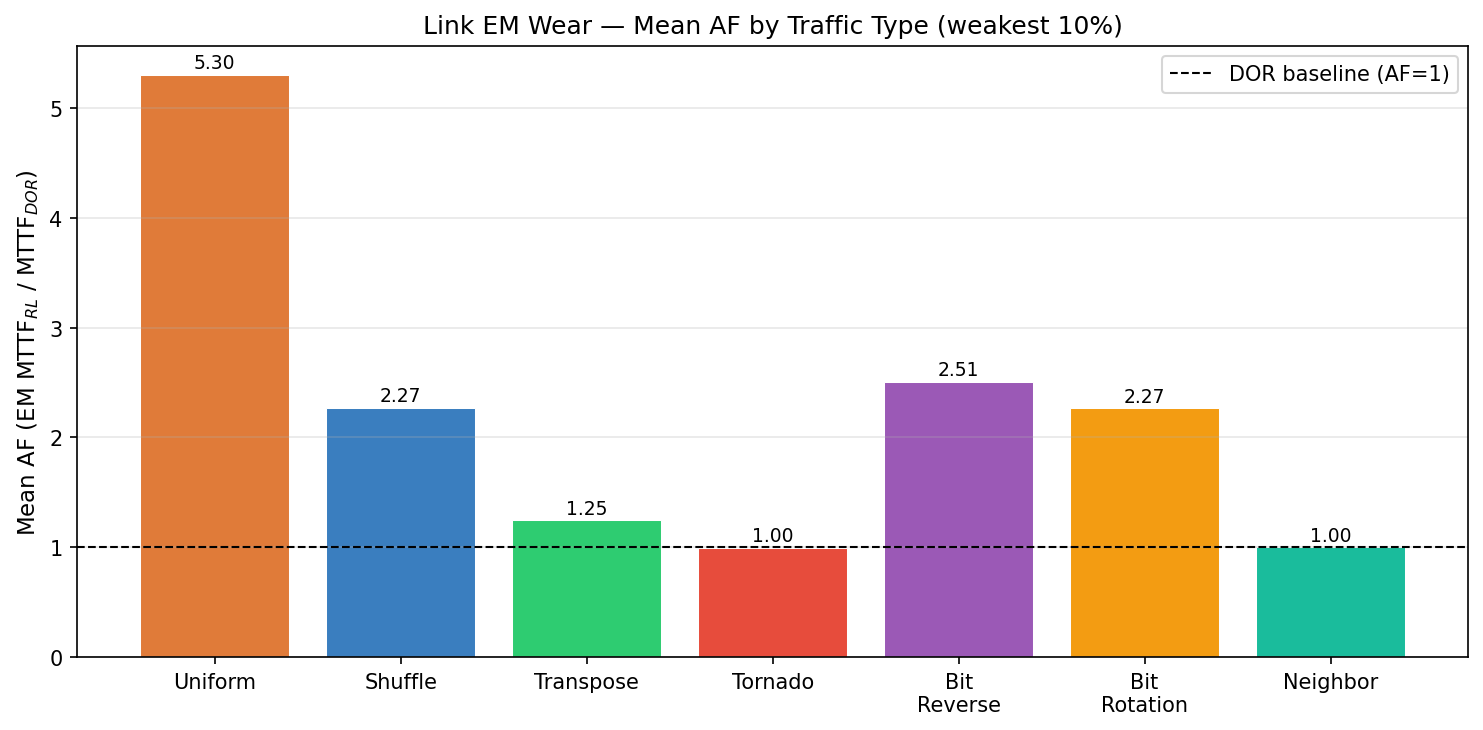
\includegraphics[width=0.95\linewidth]{body_chapters/chap_4/figs/af_weak10_bar_links.png}
      \caption[Mean EM Wear in Links]{Mean Acceleration Factor (AF) for the weakest 10\% of links under EM wear across different traffic patterns.}
      \label{fig:af_links_bar}
  \end{center}
\end{figure}

\begin{figure}[ht]
  \begin{center}
      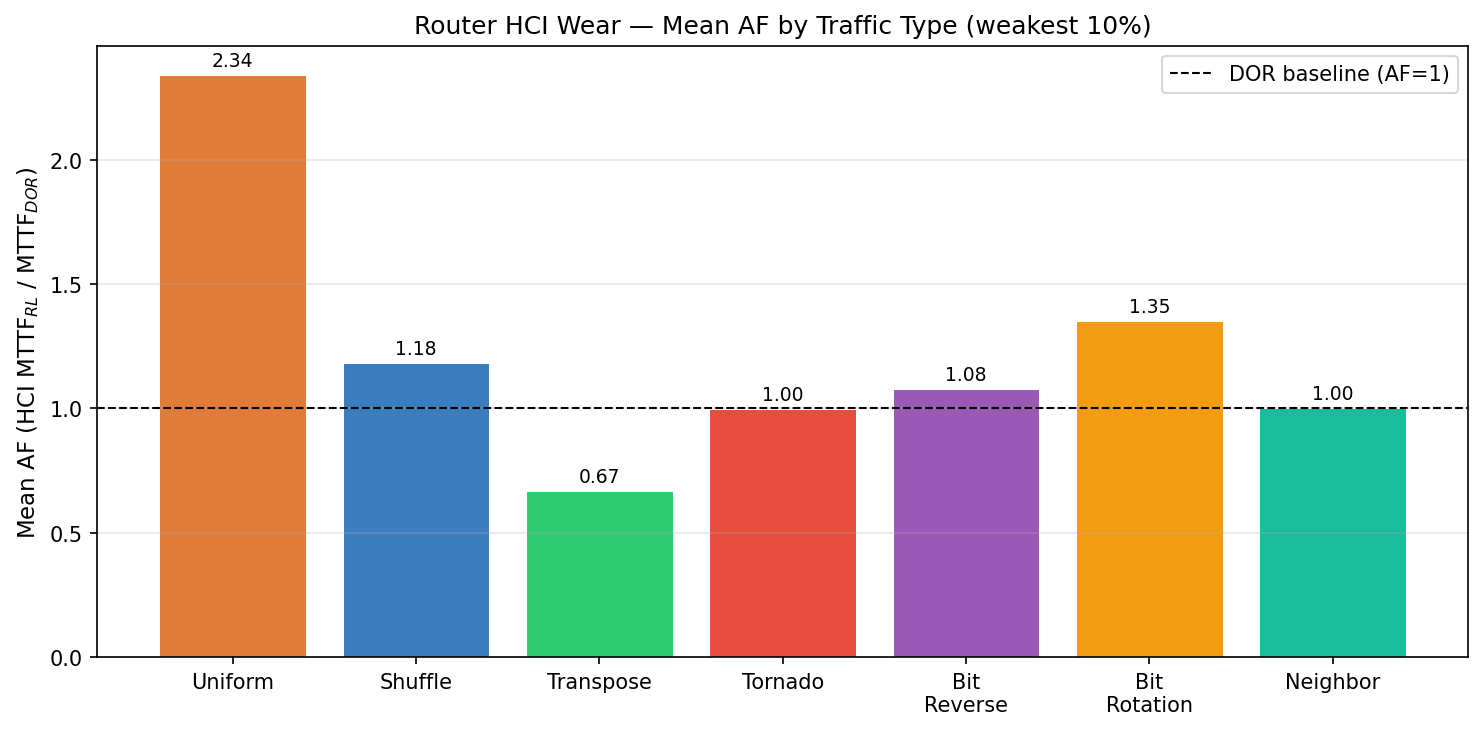
\includegraphics[width=0.95\linewidth]{body_chapters/chap_4/figs/af_weak10_bar_routers.png}
      \caption[Mean HCI Wear in Routers]{Mean Acceleration Factor (AF) for the weakest 10\% of routers under HCI wear across different traffic patterns.}
      \label{fig:af_routers_bar}
  \end{center}
\end{figure}

Overall, the proposed RL-based routing achieves significant improvements in lifetime compared to DOR, with consistently higher AF values across most traffic patterns. As expected, the improvement is more pronounced for EM than for HCI due to the quadratic dependence of EM lifetime on switching activity. Redistributing traffic away from heavily utilized links therefore yields substantial gains in EM lifetime, whereas HCI, with its linear dependence and sensitivity to process variation, exhibits more modest improvements.

For EM wear (links), the largest improvement is observed under uniform random traffic, where AF reaches approximately $5.3\times$. This reflects the ability of the RL policy to effectively balance load in a scenario with high path diversity. Shuffle and bit rotation traffic patterns yield similar improvements of approximately $2.3\times$, while bit reverse achieves around $2.5\times$. In contrast, transpose, neighbor, and tornado traffic show significantly lower gains, with AF values of approximately $1.25\times$ for transpose and close to $1.0\times$ for tornado and neighbor. This is expected, as these traffic patterns constrain packets to a limited set of shortest paths, forcing traffic through central or local links where routing flexibility is reduced.

For HCI wear (routers), a similar trend is observed, though with lower overall gains. Uniform random traffic again provides the highest improvement, with an AF of approximately $2.3\times$. Shuffle and bit rotation yield moderate improvements of around $1.2\times$. Bit reverse shows a slight improvement, while tornado and neighbor traffic exhibit little to no gain over DOR. In particular, the RL routing algorithm performs slightly worse under transpose traffic, as the routing options repeatedly stress the same set of routers along fixed shortest paths.

These results highlight two key observations. First, the effectiveness of RL-based routing is strongly dependent on the availability of path diversity. Traffic patterns that allow multiple routing choices benefit the most from adaptive routing. Second, EM benefits more than HCI due to its higher sensitivity to load redistribution, making it the dominant factor in overall lifetime improvement.

\subsubsection{Latency Analysis}

To evaluate the performance impact of the proposed routing scheme, average packet latency is measured as a function of injection rate across all traffic patterns. Representative latency curves are shown in Figures~\ref{fig:latency_curves_1}, \ref{fig:bit_rotation_latency}, \ref{fig:latency_curves_2}, \ref{fig:latency_curves_3}.

\begin{figure}[ht]
  \centering
  \begin{subfigure}{\linewidth}
    \centering
    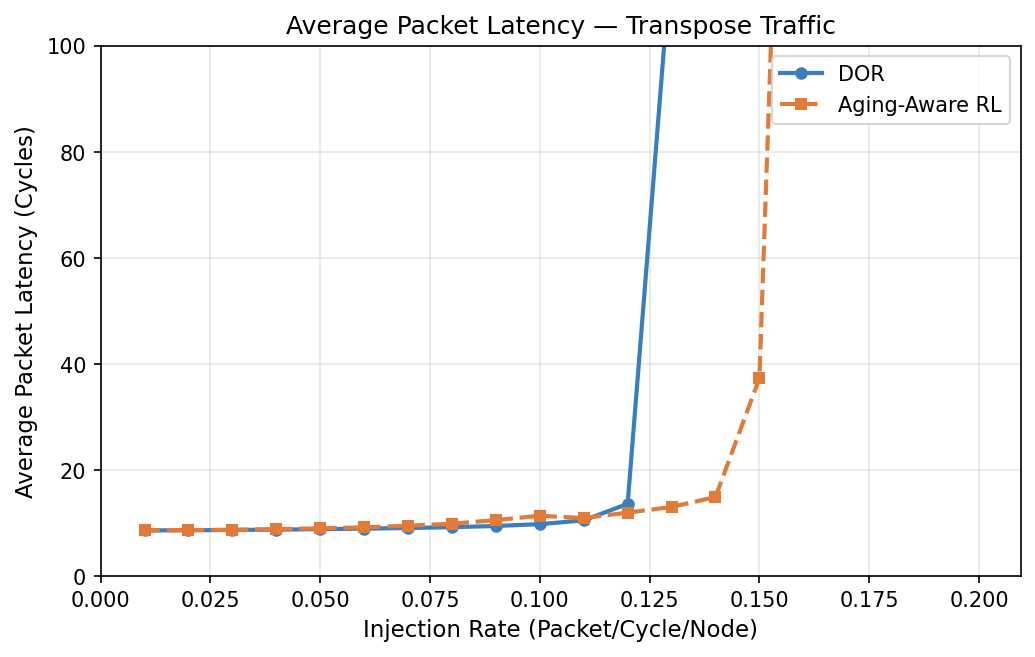
\includegraphics[width=0.8\linewidth]{body_chapters/chap_4/figs/latency_transpose.png}
    \caption{Average Packet Latency under Transpose Traffic.}
    \label{fig:transpose_latency}
  \end{subfigure}
  \vspace{1em}
  \begin{subfigure}{\linewidth}
    \centering
    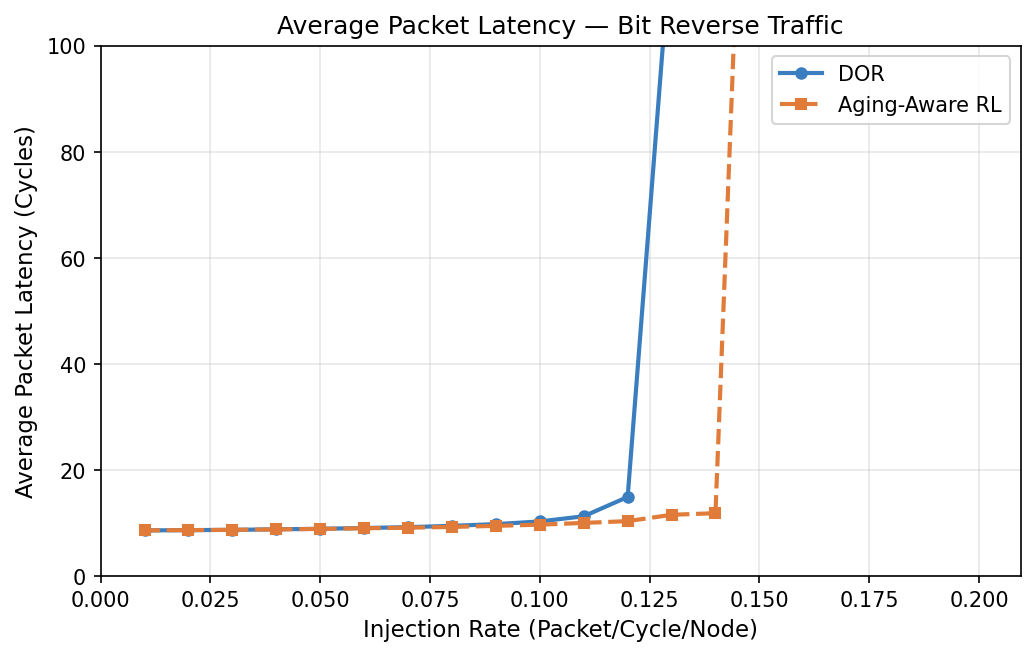
\includegraphics[width=0.8\linewidth]{body_chapters/chap_4/figs/latency_bit_reverse.png}
    \caption{Average Packet Latency under Bit Reverse Traffic.}
    \label{fig:bit_reverse_latency}
  \end{subfigure}
  \caption[Average Packet Latency (Transpose, Bit Reverse, Bit Rotation)]{Average Packet Latency vs. Injection Rate for RL-based Routing and DOR across Transpose, Bit Reverse, and Bit Rotation traffic patterns.}
  \label{fig:latency_curves_1}
\end{figure}

\begin{figure}[ht]
  \begin{center}
    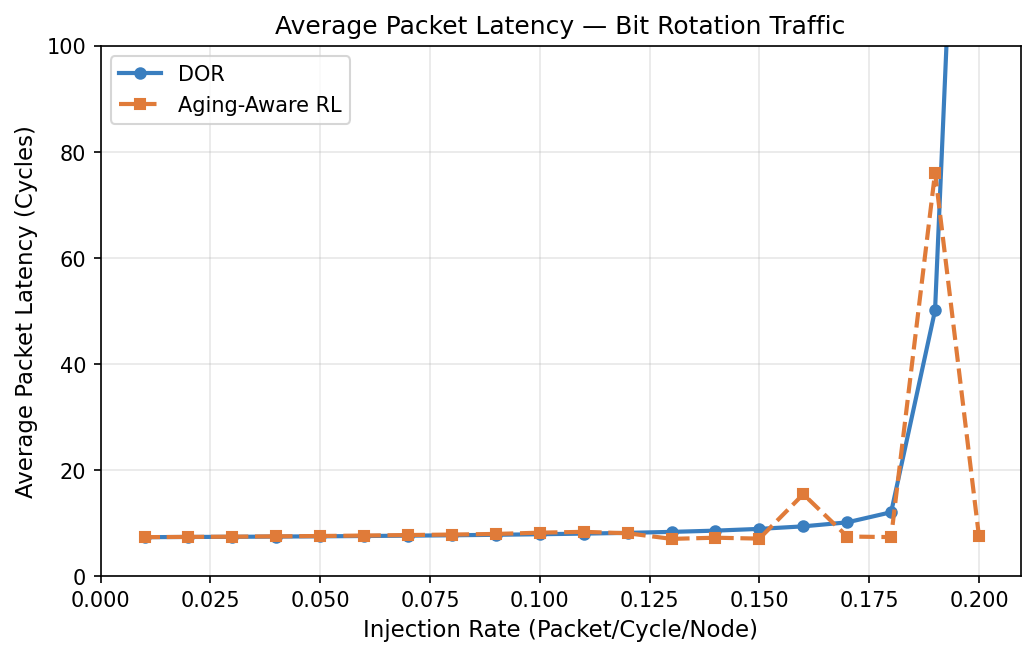
\includegraphics[width=0.8\linewidth]{body_chapters/chap_4/figs/latency_bit_rotation.png}
    \caption{Average Packet Latency under Bit Rotation Traffic.}
    \label{fig:bit_rotation_latency}
  \end{center}
\end{figure}

\begin{figure}[ht]
  \centering
  \begin{subfigure}{\linewidth}
    \centering
    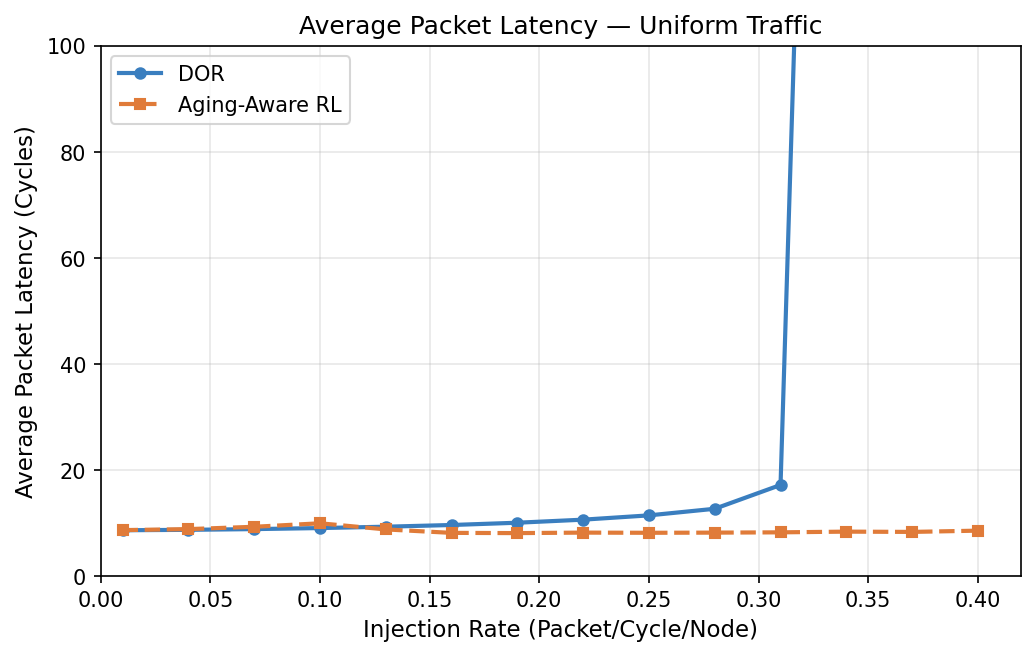
\includegraphics[width=0.8\linewidth]{body_chapters/chap_4/figs/latency_uniform.png}
    \caption{Average Packet Latency under Uniform Random Traffic.}
    \label{fig:uniform_latency}
  \end{subfigure}
  \vspace{1em}
  \begin{subfigure}{\linewidth}
    \centering
    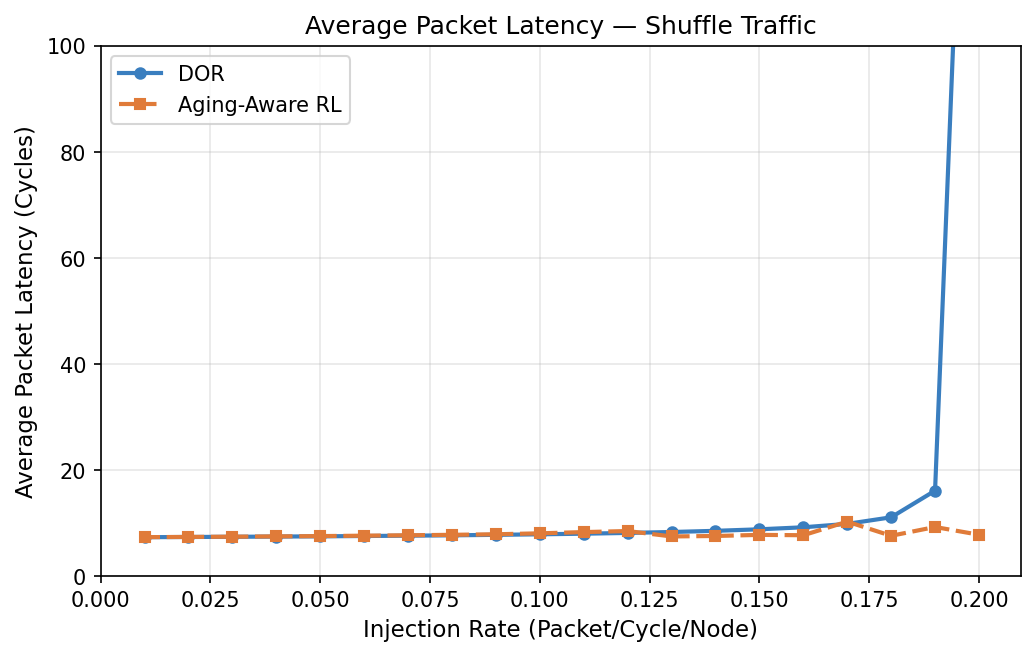
\includegraphics[width=0.8\linewidth]{body_chapters/chap_4/figs/latency_shuffle.png}
    \caption{Average Packet Latency under Shuffle Traffic.}
    \label{fig:shuffle_latency}
  \end{subfigure}
  \caption[Average Packet Latency (Uniform, Shuffle)]{Average Packet Latency vs. Injection Rate for RL-based Routing and DOR across Uniform Random and Shuffle traffic patterns.}
  \label{fig:latency_curves_2}
\end{figure}

\begin{figure}[ht]
  \centering
  \begin{subfigure}{\linewidth}
    \centering
    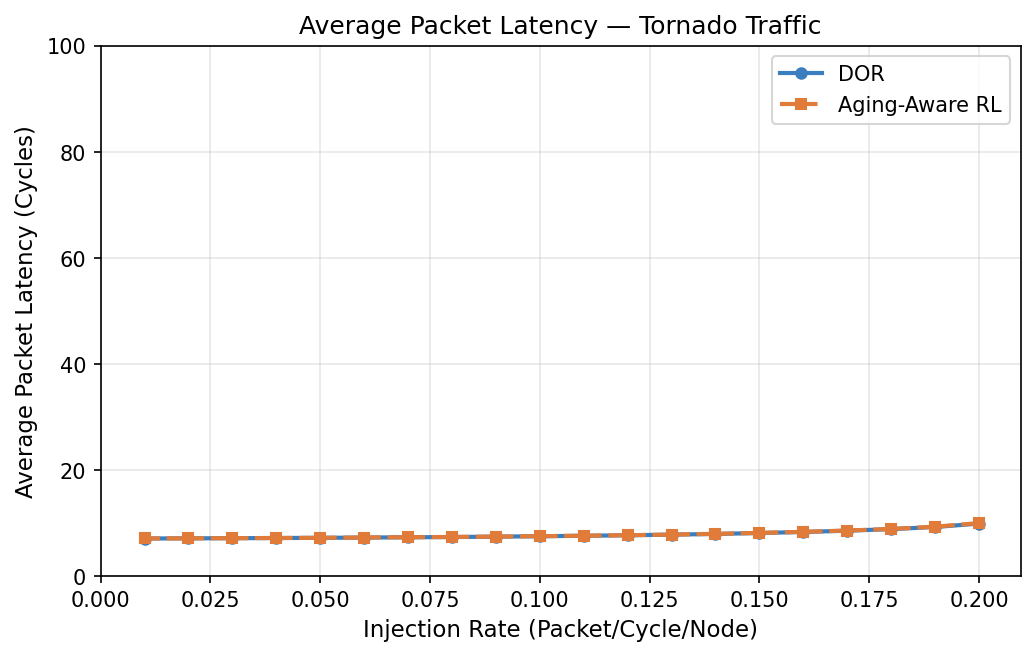
\includegraphics[width=0.8\linewidth]{body_chapters/chap_4/figs/latency_tornado.png}
    \caption{Average Packet Latency under Tornado Traffic.}
    \label{fig:tornado_latency}
  \end{subfigure}
  \vspace{1em}
  \begin{subfigure}{\linewidth}
    \centering
    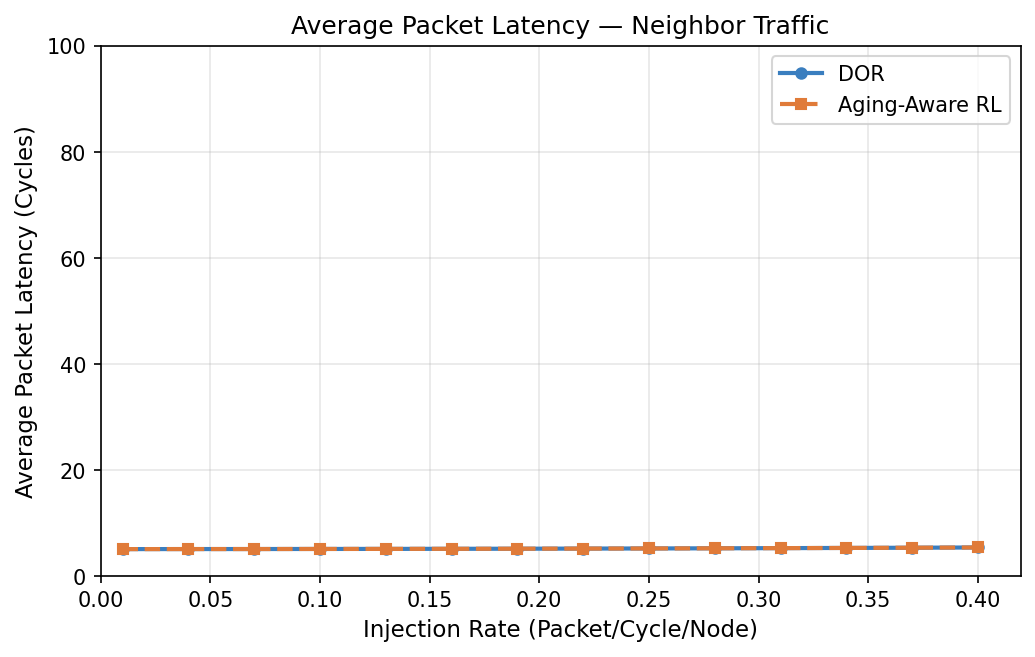
\includegraphics[width=0.8\linewidth]{body_chapters/chap_4/figs/latency_neighbor.png}
    \caption{Average Packet Latency under Neighbor Traffic.}
    \label{fig:neighbor_latency}
  \end{subfigure}
  \caption[Average Packet Latency (Tornado, Neighbor)]{Average Packet Latency vs. Injection Rate for RL-based Routing and DOR across Tornado and Neighbor traffic patterns.}
  \label{fig:latency_curves_3}
\end{figure}

Across all traffic patterns, the RL-based routing achieves latency comparable to or better than the DOR baseline. At low injection rates, both routing schemes exhibit nearly identical latency. This is expected, as the network is lightly loaded and there is limited contention, leaving little opportunity for adaptive routing to improve performance.

At higher injection rates, the benefits of RL-based routing become more apparent. As traffic increases, DOR begins to saturate due to its deterministic nature, which concentrates traffic along fixed paths and creates congestion hotspots. This results in a sharp increase in packet latency beyond the saturation point. In contrast, the RL-based routing distributes traffic more evenly across available paths, delaying the onset of congestion and maintaining lower latency under higher load conditions.

The most significant latency improvements are observed in structured traffic patterns such as bit reverse, bit rotation, shuffle, transpose, and uniform random. These patterns provide multiple routing options, allowing the RL agent to effectively balance load and avoid congested regions. In these cases, RL not only improves reliability but also enhances network performance.

For neighbor and tornado traffic, both routing schemes exhibit similar latency. This is expected, as these patterns constrain packets to a limited set of shortest paths, leaving little flexibility for adaptive routing to redistribute traffic. As a result, RL does not provide a noticeable performance advantage in these scenarios, but importantly, it does not degrade performance either.

% This is a reference to a label in another chapter. Appendix~\ref{chap:app1}. You can always refer to other labels from other chapters with the \textbf{\textbackslash ref} command. 

% It is good practice to follow the latex prefix guidelines for label names:
% \begin{itemize}
%     \item \textit{ch}:	chapter
%     \item \textit{sec}:	section
%     \item \textit{subsec}:	subsection
%     \item \textit{fig}:	figure
%     \item \textit{tab}:	table
%     \item \textit{eq}:	equation
%     \item \textit{lst}:	code listing
%     \item \textit{itm}:	enumerated list item
%     \item \textit{alg}:	algorithm
%     \item \textit{app}:	appendix subsection
% \end{itemize}



% \section{Summary}
% \lipsum[5]
% \section{Future Work}
% \lipsum[6]


% Insert the bibliography
\bibliographystyle{unsrt} % We choose the "unsrt" reference style
\bibliography{sample_bib} % Entries are in the sample_bib.bib file

% ========================================
% APPENDICES
% ========================================
\appendix
% Add as many of the following statements as you need. 
\chapter{Mean Acceleration Factor}
\label{chap:app1}

\section{Mean Acceleration Factor (AF) Trends Across Injection Rates}

\begin{figure}[ht]
  \begin{center}
      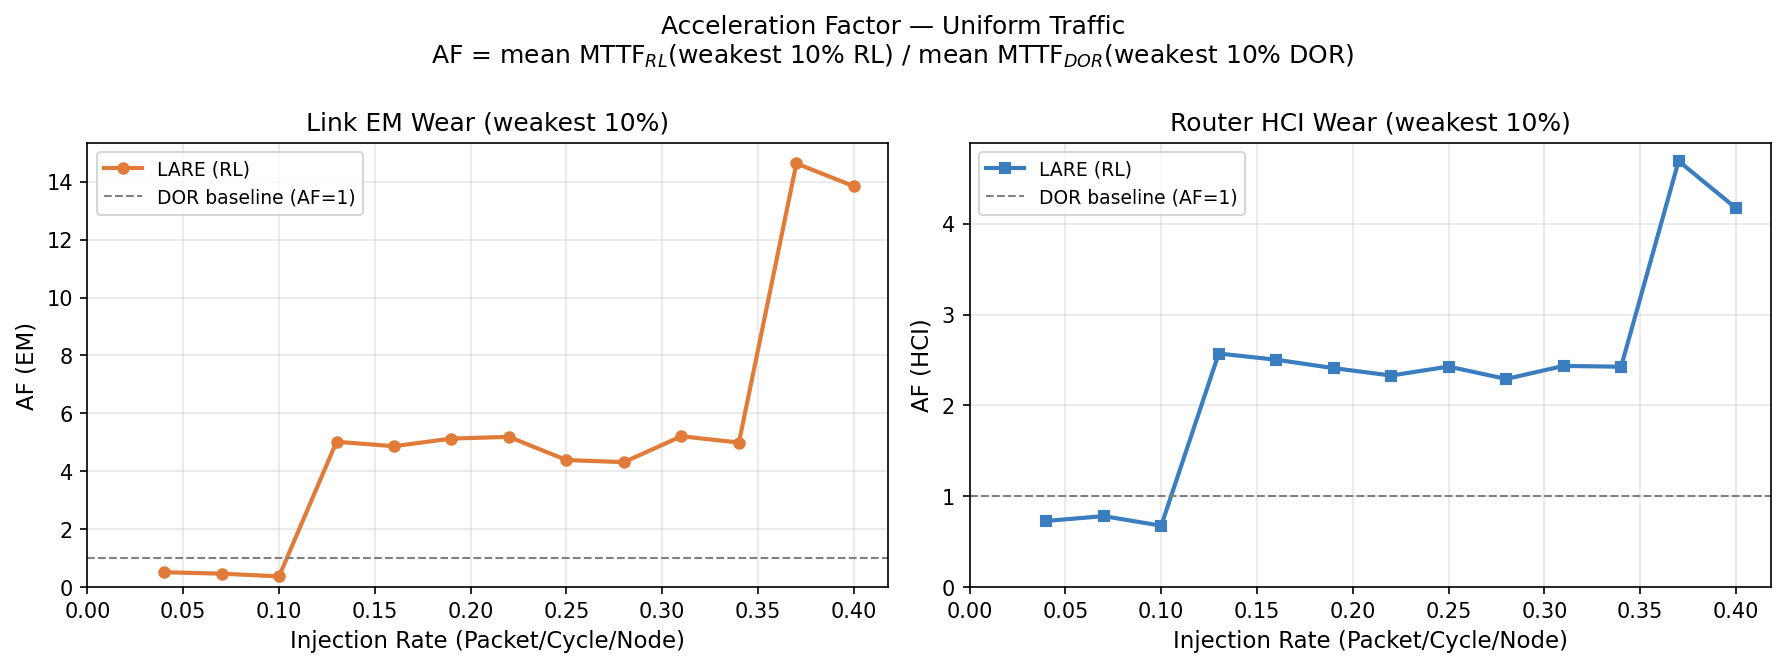
\includegraphics[width=1\linewidth]{body_chapters/chap_a1/figs/uniform.png}
      \caption[Uniform Random Traffic.]{Mean Acceleration Factor (AF) for uniform random traffic across different injection rates.}
      \label{fig:uniform_af}
  \end{center}
\end{figure}

\begin{figure}[ht]
  \begin{center}
      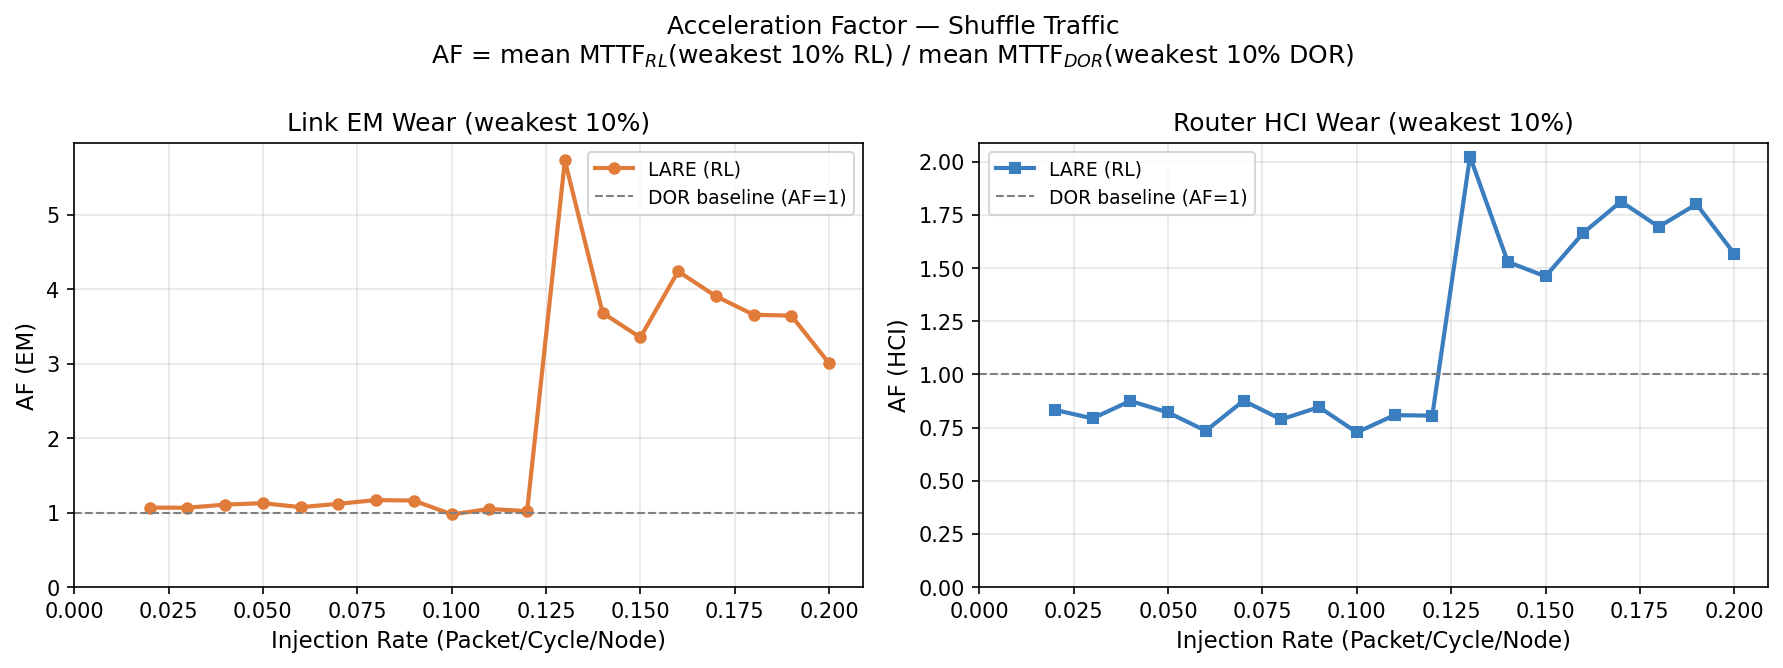
\includegraphics[width=1\linewidth]{body_chapters/chap_a1/figs/shuffle.png}
      \caption[Shuffle Traffic.]{Mean Acceleration Factor (AF) for shuffle traffic across different injection rates.}
      \label{fig:shuffle_af}
  \end{center}
\end{figure}

\begin{figure}[ht]
  \begin{center}
      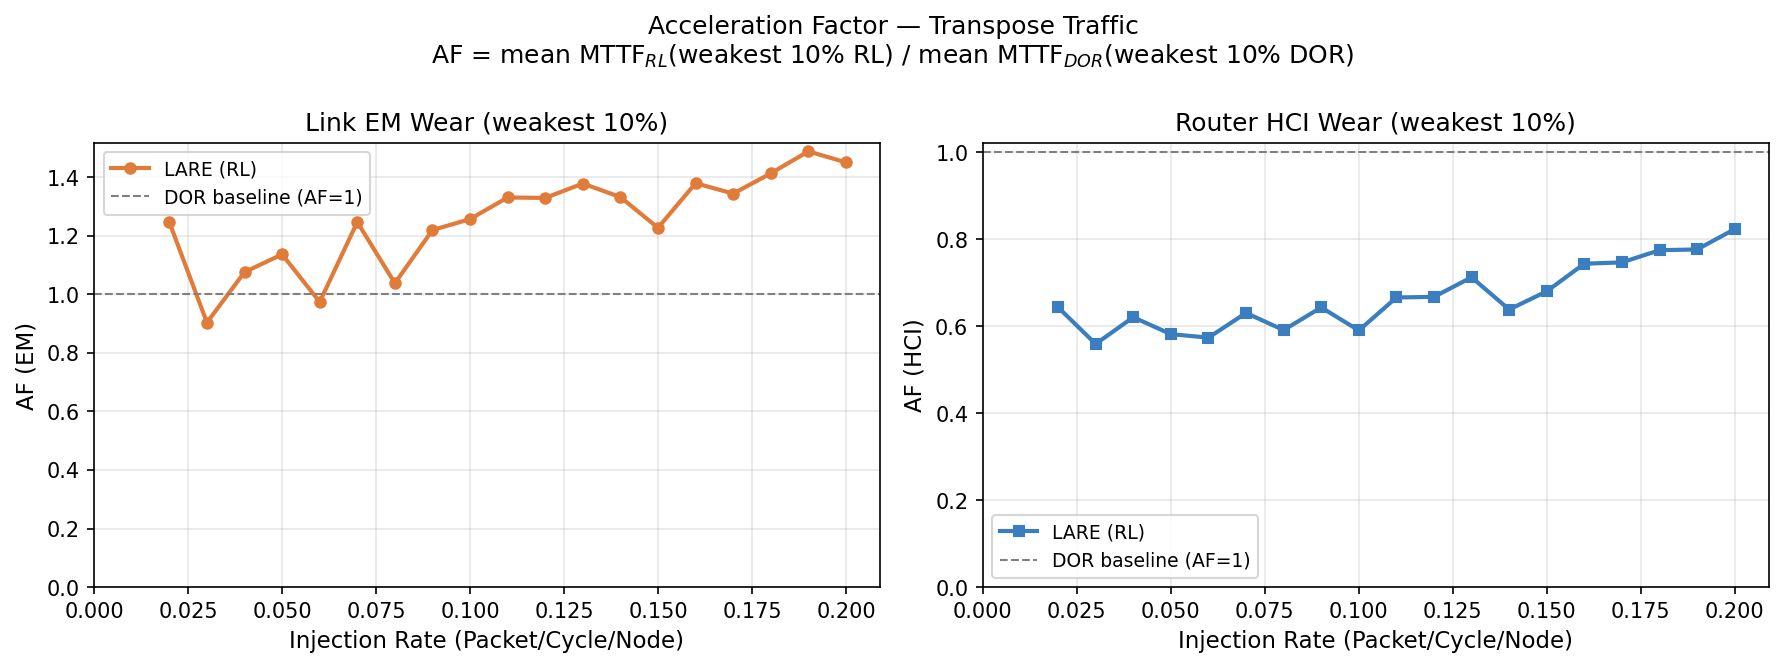
\includegraphics[width=1\linewidth]{body_chapters/chap_a1/figs/transpose.png}
      \caption[Transpose Traffic.]{Mean Acceleration Factor (AF) for transpose traffic across different injection rates.}
      \label{fig:transpose_af}
  \end{center}
\end{figure}

\begin{figure}[ht]
  \begin{center}
      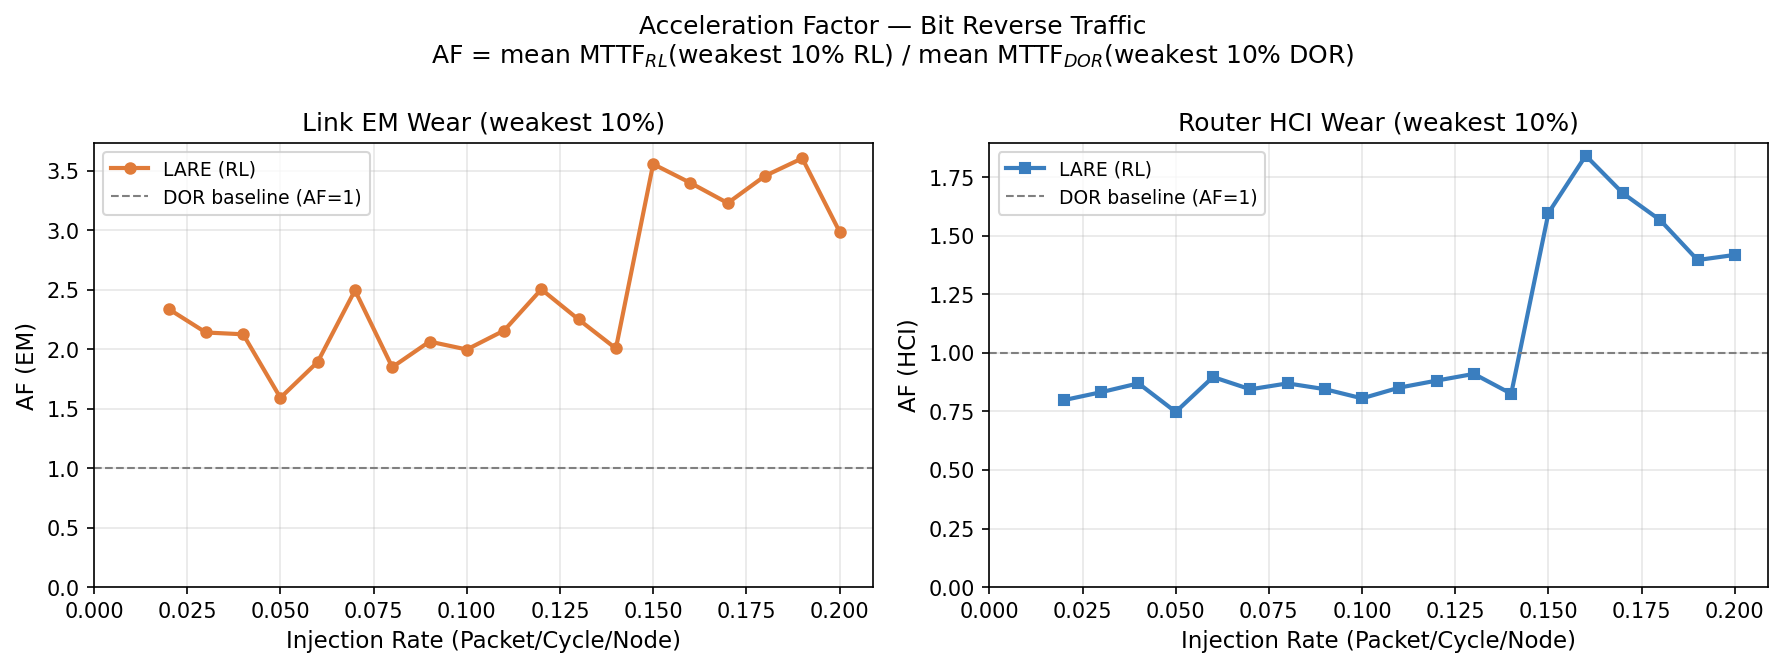
\includegraphics[width=1\linewidth]{body_chapters/chap_a1/figs/bit_reverse.png}
      \caption[Bit Reverse Traffic.]{Mean Acceleration Factor (AF) for bit reverse traffic across different injection rates.}
      \label{fig:bit_reverse_af}
  \end{center}
\end{figure}

\begin{figure}[ht]
  \begin{center}
      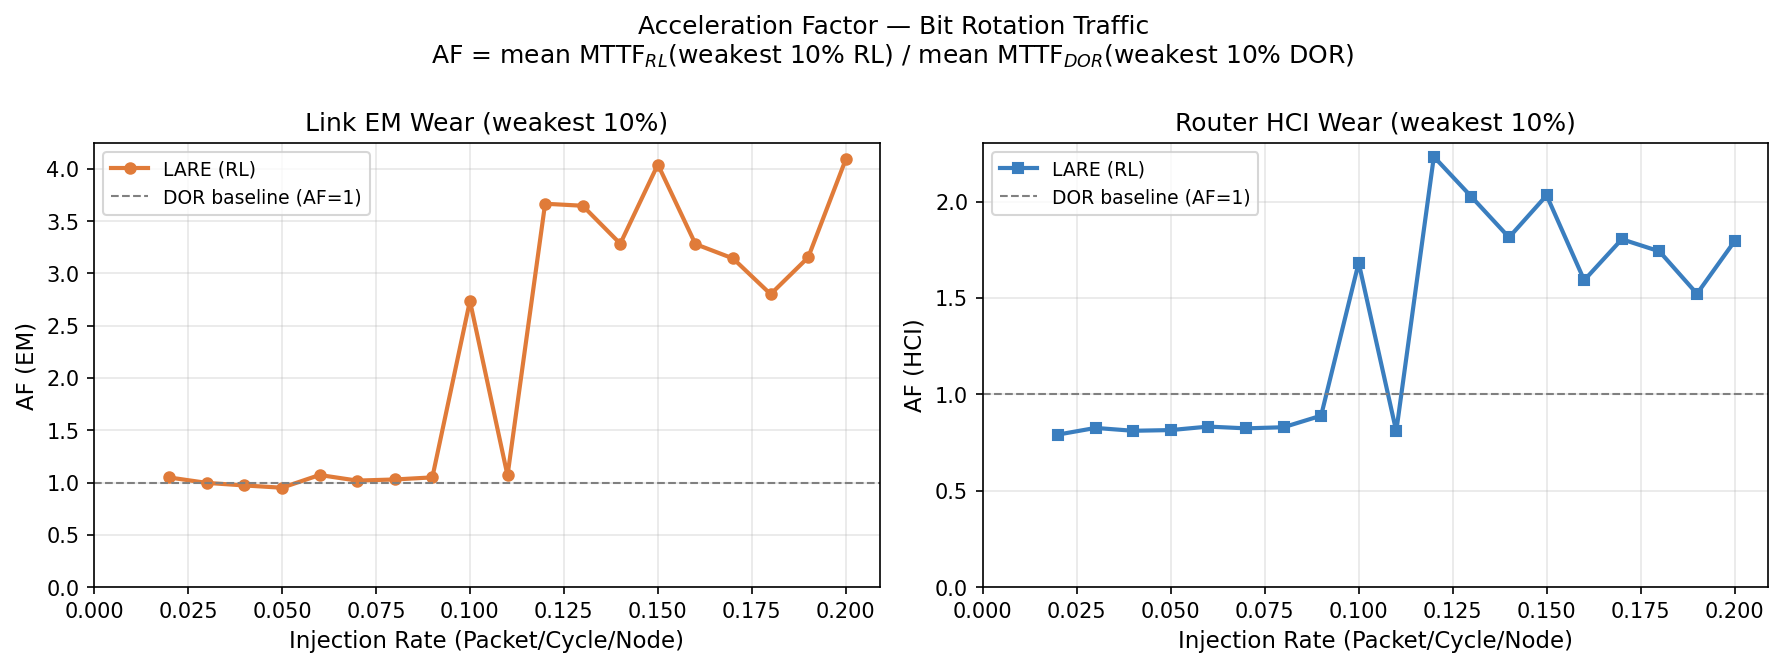
\includegraphics[width=1\linewidth]{body_chapters/chap_a1/figs/bit_rotation.png}
      \caption[Bit Rotation Traffic.]{Mean Acceleration Factor (AF) for bit rotation traffic across different injection rates.}
      \label{fig:bit_rotation_af}
  \end{center}
\end{figure}

\begin{figure}[ht]
  \begin{center}
      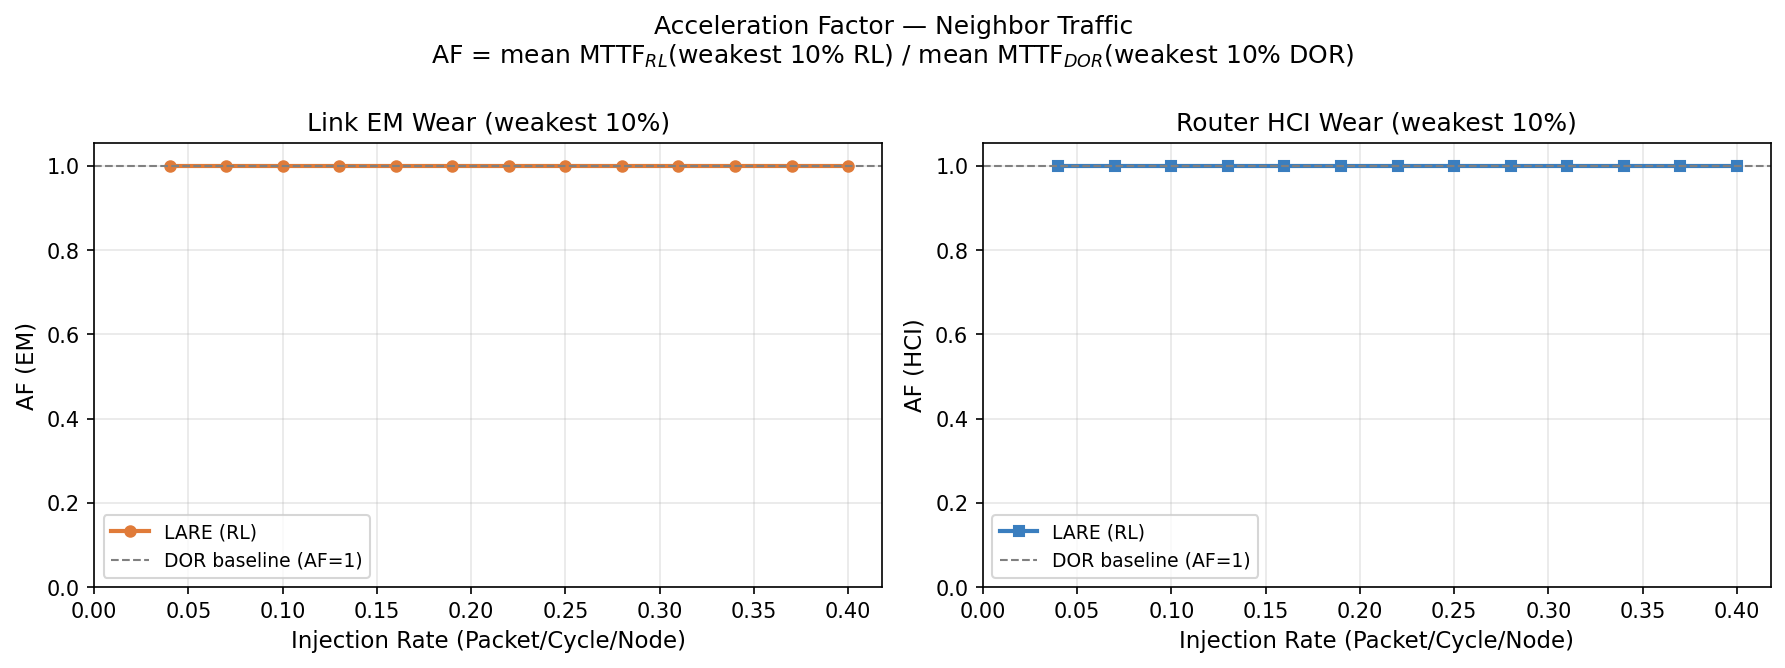
\includegraphics[width=1\linewidth]{body_chapters/chap_a1/figs/neighbor.png}
      \caption[Neighbor Traffic.]{Mean Acceleration Factor (AF) for neighbor traffic across different injection rates.}
      \label{fig:neighbor_af}
  \end{center}
\end{figure}

\begin{figure}[ht]
  \begin{center}
      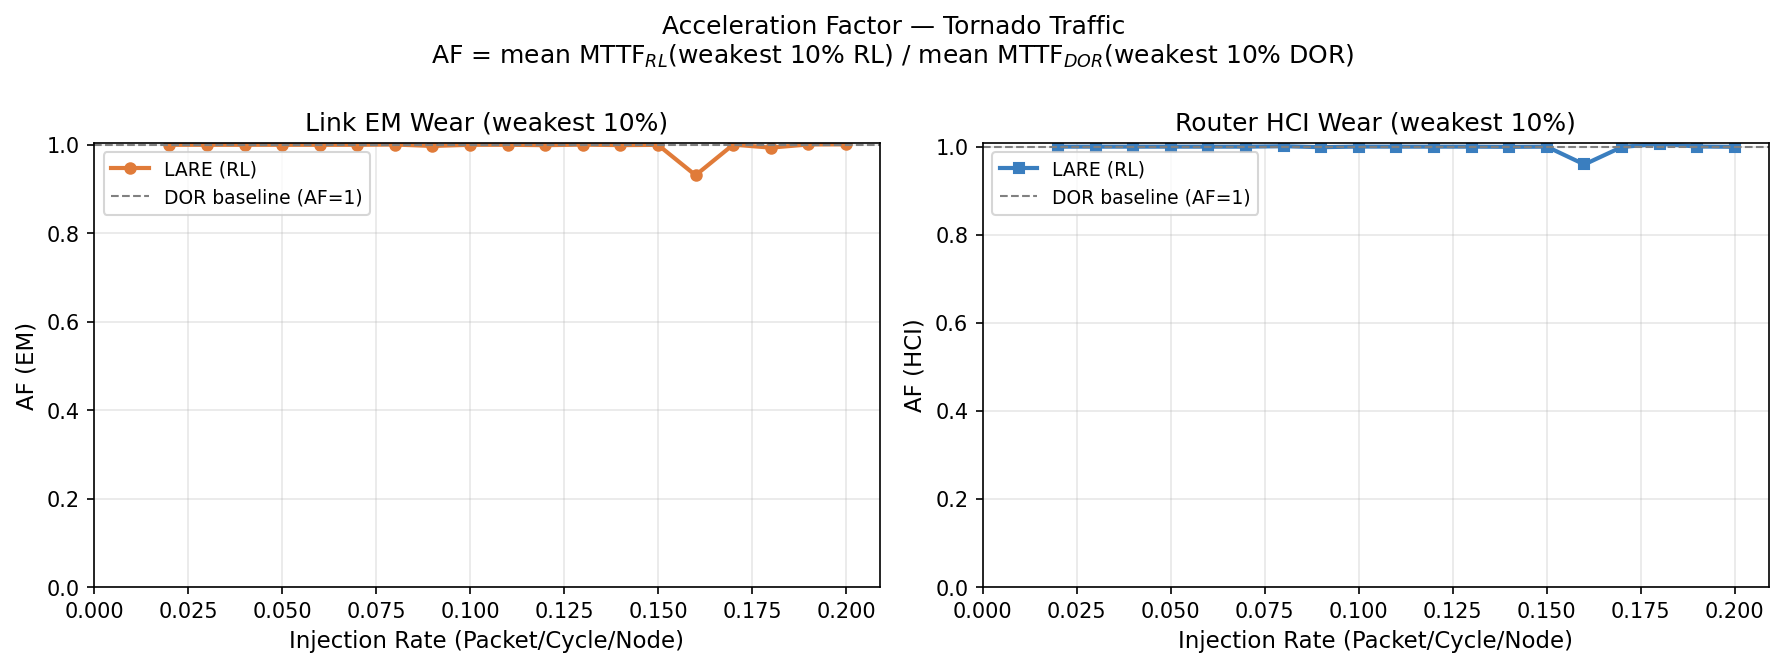
\includegraphics[width=1\linewidth]{body_chapters/chap_a1/figs/tornado.png}
      \caption[Tornado Traffic.]{Mean Acceleration Factor (AF) for tornado traffic across different injection rates.}
      \label{fig:tornado_af}
  \end{center}
\end{figure}
% \chapter{Access to Research Work}

\section{Code}

The code and relevant documentation for this thesis are available at the following GitHub repository: \url{https://github.com/IshraqF/CPEN-499-Thesis.git}. This repository includes all source code, scripts, and data used in the experiments and analyses presented in this thesis. The repository is organized into directories corresponding to the simulator, the thesis report, and the thesis logbook, ensuring that all materials are easily accessible for review and replication of results.



\end{document}